\documentclass[Times,12pt,oneside,openany,print,index]{report}
\usepackage[a4paper,width=150mm,top=25mm,bottom=25mm]{geometry}
\usepackage[english]{babel}
\usepackage[utf8]{inputenc}
\usepackage{csquotes} % Provides advanced facilities for in-line and display quotations
\usepackage{amsmath} % TO use mathematical equations 
\pagestyle{plain} % Just a plain page number. For more http://www.emerson.emory.edu/services/latex/latex_129.html

\usepackage{graphicx} % to use the graphicx package
\graphicspath{/images} % Path to Image files 
\usepackage{caption} % To use caption with figure and images
\usepackage{array} % The array environment is used to make a table of information, with column alignment (left, center, or right) and optional vertical lines separating the columns

\usepackage[pdftex]{hyperref}
\usepackage{multirow}
\usepackage{booktabs}
\usepackage{graphicx}
\usepackage[nottoc]{tocbibind} % The tocbibind package can be used to add the ToC and/or bibliography and/or the index etc., to the Table of Contents listing

\usepackage[normalem]{ulem} % The ulem package provides various types of underlining that can stretch between words and be broken across lines.

\usepackage{hyperref} % Provides LaTeX the ability to create hyperlinks within the document.
\usepackage[document]{ragged2e}
\usepackage{hyperref}
\hypersetup{
    colorlinks=true,
    linkcolor=black,
    filecolor=magenta,      
    urlcolor=black,
    citecolor=black,
}
\urlstyle{same}

\setlength{\parindent}{0em} % To control Indentation of paragraphs 

\usepackage{nomencl} % The nomenclature package can be used to generate and format a nomenclature using MakeIndex.
\renewcommand{\nompreamble}{The next list describes several symbols \& abbreviation that will be later used within the body of the document}
\makenomenclature


\usepackage[backend=biber,style=ieee,sorting=ynt]{biblatex} % for more plz click https://www.overleaf.com/learn/latex/Biblatex_citation_styles
\addbibresource{bibliography/references.bib} % Imports bibliography file

\let\cleardoublepage=\clearpage % removes unwanted doublepages
\begin{document}
\justifying
\thispagestyle{empty} % removes page number from title page
\begin{titlepage}
\renewcommand*{\thepage}{Title} % Change page number in PDF

    \begin{center} 
        \vspace*{3cm} % For creating Vertical Blank Space
        
        {\fontsize{16pt}{22pt}\selectfont{Decipherable Classification of Glaucoma using\\
        Deep Neural Network Leveraging XAI}
        } % "fontsize{font size}{line space}\selectfont{}" command to override font size and line space for the Title
        
        \vspace{1.5cm}
        
        \text{by}
        
        \vspace{0.5cm}
        
        	Touhidul Islam Chayan\\
	        17101362\\
	        Anita Islam\\
	        17301021\\
	        Anika Rahman Tonny\\
	        18101569\\
	        Eftykhar Rahman\\
	        18301041

        \vspace{1.5cm}
        
        	A thesis submitted to the Department of Computer Science and Engineering\\
            in partial fulfillment of the requirements for the degree of\\
            B.Sc. in Computer Science and Engineering

        
        \vspace{2.5cm}
        
    		Department of Computer Science and Engineering\\
            Brac University\\
            January 2022
        
        \vspace{3cm}
        
    		\copyright\ 2022. Brac University\\
            All rights reserved.
    
    \end{center}

\end{titlepage} % Add title page
\cleardoublepage

\pagenumbering{roman} % Roman numbers to be use all pages before Chapter 1

%*******************************************************************
% TOC = Table of Contents
% The hyperref makes Title page No. 1 entry in the TOC
% In order to properly link  all section in TOC "phantomsection" command used
%  see below link for details on "addcontentsline"
% http://www.emerson.emory.edu/services/latex/latex_162.html
% "input" command to add files
% "Ethics Statement" & "Dedication" page are Optional; you may omit this two page if you want
% Please do not change the order of listings in TOC
%*******************************************************************
\phantomsection
\addcontentsline{toc}{chapter}{Declaration}
% Following command is used to created grouped signature line for Four Authors
\newcommand*\wildcard[2][6cm]{\vspace{2cm}\parbox{#1}{\hrulefill\par#2}} 

% A "parbox{}{}" is a box whose contents are created in paragraph mode. 
% "hrulefill{} to chance thickness of underline"

\section*{Declaration}

It is hereby declared that

\begin{enumerate} % begin{enumerate} function to create numbered list
  \item The thesis submitted is my/our own original work while completing degree at Brac University.
  \item The thesis does not contain material previously published or written by a third party, except where this is appropriately cited through full and accurate referencing.
  \item The thesis does not contain material which has been accepted, or submitted, for any other degree or diploma at a university or other institution.
  \item We have acknowledged all main sources of help.
\end{enumerate}

\vspace{1cm}
\textbf{Student’s Full Name \& Signature:} % Testbf{} for Bold

\begingroup
    \begin{center}
        
        \wildcard{\centerline{Touhidul Islam Chayan} \\ \centerline{17101362}} 
        \hspace{2cm}
        \wildcard{\centerline{Anita Islam} \\ \centerline{17301021} }
        \wildcard{\centerline{Anika Rahman Tonny} \\ \centerline{18101569} }
        \hspace{2cm}
        \wildcard{\centerline{Eftykhar Rahman \\} \\ \centerline{18301041} }
    \end{center}
\endgroup


\pagebreak







\phantomsection
\addcontentsline{toc}{chapter}{Approval}
\section*{Approval}

The thesis/project titled “Decipherable Classification of Glaucoma using Deep Neural Network Leveraging XAI” submitted by 
\begin{enumerate}
  \item Touhidul Islam Chayan (17101362)
  \item Anita Islam (17301021)
  \item Anika Rahman Tonny (18101569) 
  \item Eftykhar Rahman (18301041)
\end{enumerate}

\noindent Of Fall, 2021 has been accepted as satisfactory in partial fulfillment of the requirement for the degree of B.Sc. in Computer Science and Engineering on January 18, 2022. 

\noindent \textbf{Examining Committee:}

\noindent Supervisor:\\
\noindent (Member)
\begin{center}
\begin{figure}[hbt!]
\raggedleft

\includegraphics[scale=0.3]{images/tanjimRezaSir.png}\ \ \ \ \ \ \ \ \ \ \ \ \ \ \ \ \ \
\end{figure}    
    \hspace{7cm} \wildcard{\centerline{MD Tanzim Reza} \\ \centerline{Lecturer}\\ \centerline{Computer Science and Engineering}\\ \centerline{Brac University} } \hspace{1cm} 
\end{center}

\noindent Program Coordinator:\\
(Member)
\begin{center}
    % \hspace{7cm} Md. Golam Rabiul Alam \\
    \hspace{7cm} \wildcard{\centerline{Md. Golam Rabiul Alam, PhD} \\ \centerline{Associate Professor} \centerline{Computer Science and Engineering}\\ \centerline{Brac University} } \hspace{1cm} 
\end{center}

\noindent Head of Department:\\
(Chair)
\begin{center}
    % \hspace{7cm} Sadia Hamid Kazi \\
    \hspace{7cm} \wildcard{\centerline{Sadia Hamid Kazi} \\ \centerline{Chairperson and Associate Professor}\\ \centerline{Department of Computer Science and Engineering }\\ \centerline{Brac University} } \hspace{1cm} 
\end{center}

\pagebreak

\phantomsection
\addcontentsline{toc}{chapter}{Ethics Statement}
\section*{Ethics Statement}
We, the members, hereby and genuinely declare that this thesis is based on our thorough study findings. This report appropriately notes and cites all of the materials that were utilized. This research work, in its entirety or in part, has never been submitted to another university or institution for the purpose of awarding a degree or for any other purpose.
\pagebreak

\phantomsection
\addcontentsline{toc}{chapter}{Abstract}
\section*{Abstract}
Glaucoma is the second driving reason for partial or complete blindness among all the visual deficiencies which mainly occurs because of excessive pressure in the eye due to anxiety or depression which damages the optic nerve and creates complications in vision. In this research, we used the Glaucoma Dataset in our algorithm to predict outcomes related to Glaucoma and non-glaucoma. The main goal of the author of this research was to develop an automated deep learning neural network architecture for early detection of Glaucoma disease. For the classification of glaucoma two Black Box models have been used in the paper. Fully Connected Neural Network (FCNNs) which is a Conventional Neural Network (CNN) composed of a fully connected layer. These Deep FCNN Black Box models have been described through Explainable Artificial Intelligence (XAI) to achieve the ultimate goal of our research. However, to serve our purpose we have used VGG-16, VGG-19, DenseNet121, InceptionV3 and ResNet50 Deep FCNNs models for our study. To begin with we pre-processed the images and grouped them into three sets: training, testing and validation. Afterwards, These models have been initialized with the pre-existing models trained on the imagenet dataset. Conclusively, the training and evaluating of all the Deep FCNN has been done. The validation accuracy of our models we got are as follows: In InceptionV3 we got 86.4\% accuracy, in DenseNet121 we got 86.8\% accuracy, in ResNet50 we got 94.7\% accuracy, in VGG-19 we got 93.3\% accuracy and lastly in VGG-16 we got 88.6\% accuracy. As follows, after 50 epochs,  ResNet50 got the highest score among the other models with a validation accuracy of 94.7\%. Afterwards, we compared all models' accuracy and loss graph together, where we can see that VGG-19 and ResNet50 were the Good-Fit than the other models. As a result, our research achieved outstanding classification accuracy in a short period of time. However, it seems to be vital to understand that a human can rely on black-box level Deep Learning Models to make decisions. Throughout this work, a hybrid approach combining image processing with deep learning has been used with the support of  XAI to assure reliable glaucoma detection at an early stage.

\vspace{1cm}
\noindent \textbf{Keywords:} Glaucoma, Blindness, Diagnosis, Neural Network, XAI, Goal.
\pagebreak


% \phantomsection
% \addcontentsline{toc}{chapter}{Dedication}
% \section*{Dedication (Optional)}
A dedication is the expression of friendly connection or thanks by the author towards another person. It can occupy one or multiple lines depending on its importance.
You can remove this page if you want.

\pagebreak

\phantomsection
\addcontentsline{toc}{chapter}{Acknowledgment}
\section*{Acknowledgement}
Firstly, all praise to the Great Allah for whom our thesis have been completed without any major interruption.\\
Secondly, to our supervisor MD Tanzim Reza sir for his kind support and advice in our work. He helped us whenever we needed help.\\
And finally to our parents without their throughout support it may not be possible. With their kind support and prayer we are now on the verge of our graduation.

\renewcommand{\contentsname}{Table of Contents} % Rename TOC name from Contents to Table of Contents
\cleardoublepage
\phantomsection
\addcontentsline{toc}{chapter}{Table of Contents} % Add Table of Contents in TOC
\tableofcontents % To  generation of the Table of Contents

\listoffigures % To  generation of the List of Figure
\listoftables % To  generation of the Tables of Figure

\printnomenclature % TO  generation of the Nomenclature file
\addcontentsline{toc}{chapter}{Nomenclature}
\cleardoublepage

\pagenumbering{arabic} % To use page number 1,2,3 ..

\chapter{Introduction}
%\section{Introduction}
\section{Motivation} 
Glaucoma is one of the most painful diseases caused by excessive levels of pressure in the eyes which creates a permanent loss of vision. It is also known as the ‘silent thief of sight’ as it cannot be detected at an early stage [1]. Around 57.5 million people worldwide are affected with Glaucoma. We are going to use Explainable AI (XAI) to classify scanned images of eyes that have glaucoma. XAI proposes the report to the decision of Artificial Intelligence which means Deep Learning or to the extent that it can be interpreted by humans, it's a black box. Artificial Intelligence (AI) has a subset called Deep Learning (DL) dependent on profound neural networks which have made striking leaps forwards in clinical imaging, especially for image characterization and pattern acknowledgment [2]. The use of Deep Learning (DL) is increasing in glaucoma research because these models can accomplish high precision, issues with trust, interpretability, and experimental utility structure hindrances to occurring clinical practice. The main goal of this research is to represent whether and how deep learning-based measurements can be utilized for glaucoma execution in the clinic [3]. Unfortunately, not many people bother about the early detection of Glaucoma whereas it can be diagnosed early to prevent eyesight loss. For this reason, we have decided to work with early detection of glaucoma disease to contribute to society for the good.

\section{Introduction}
Glaucoma is an eye illness wherein the optic nerve is harmed prompting irreversible loss of vision because of excessive pressure in eyes. The ciliary body emits fluid humor into the posterior chamber, which is the gap between the iris and the focus point, which is created by the eye. It then travels through the pupil and into the first chamber between the iris and cornea. It then leaves the eye after passing through a wipe-like design at the iris's base, known as the trabecular meshwork. In a solid eye, the rate at which discharge adjusts the rate of seepage. In individuals with glaucoma, the seepage waterway is part of the way or totally hindered. Liquid develops in the chambers and this expands pressure inside the eye. The pressing factor drives the focal point back and pushes on the glassy body which thus packs and harms the veins and nerve strands running at the rear of the eye. These harms bring about patches of vision misfortune, and whenever left untreated, may prompt absolute visual impairment. Glaucoma is divided into two types: First one is open-angle and second one is angle-closure.

\vspace{5mm}
\noindent Open-angle glaucoma is brought about by an incomplete blockage of the waste trench. The point between the cornea and the iris is- open, which means the passageway to the waterway is clear, however, the progression of watery humor is more slow than typical. The pressing factor develops continuously in the eye throughout a significant period. Side effects show up continuously, beginning from fringe vision misfortune, and may go on unseen until focal vision is influenced. Movement of glaucoma can be halted with medicines, however, part of the vision that is now lost can’t be reestablished. This is the reason it’s vital to distinguish early indications of glaucoma with standard eye tests.

\vspace{5mm}
\noindent Angle-closure glaucoma brought about by an abrupt and complete blockage of fluid humor waste. The pressing factor inside the eye rises quickly and may prompt absolute visual deficiency rapidly. Certain anatomical highlights of the eye, for example, limited seepage point, shallow foremost chamber, slender and saggy iris, make it simpler to foster intense glaucoma. Commonly, this happens when the understudy is expanded and the focal point has adhered to the rear of the iris. This squares the fluid humor from coursing through the understudy into the foremost chamber. Collection of liquid in the back chamber pushes on the iris, making it swell outward and square the waste point. Acute angle-closure glaucoma is a visual crisis and requires quick consideration through early detection.

\vspace{5mm}
\noindent Glaucoma, on the other hand, is one of the primary causes of blindness in people over 60. Statistics show that even with the treatment 15\% to 20\% of patients become blind. For this reason, in this research, we are going to apply Explainable AI to detect Glaucoma in a better way than exists. As the diagnosis of glaucoma is a complicated and expensive process, the application of a Deep Neural network leveraging XAI can give more improvement in understanding or detecting many problems related to glaucoma disease.


\section{Research Objectives}
The field of Explainable Artificial Intelligence has filled dramatically lately with innovations, techniques, and applications arising at a fast rate. A considerable lot of these progressions have been utilized to improve the conclusion and the executives of glaucoma. We intend to give an outline of ongoing distributions in regards to the utilization of man-made consciousness to improve the recognition and treatment of glaucoma.

\vspace{5mm}
\noindent According to modern medical science, glaucoma is diagnosed in four different ways. Initially, glaucoma is diagnosed by machine where the pressure is measured inside the eye. Here the whole diagnostic test is called Tonometry and the intraocular pressure is measured throughout this process. Apart from this, there is a prerequisite of this test which is a visual feel check. In this investigation, the doctor will move his hand from top to bottom, bottom to top, left to right, and right to left while the patient will close their eyes during the test. In this way, the doctor checks the patient’s visibility through one eye.

\vspace{5mm}
\noindent Moreover, there is another way of diagnosing glaucoma which is the Imaging Test where the main motive is to check the depth of eyes by showing pictures. However, the final diagnosis is pachymetry where The definitive diagnosis, however, is pachymetry, which is a medical gadget that measures the thickness of the cornea of the eye. In the above ways, glaucoma can be diagnosed and partial or complete blindness could be prevented.

\vspace{5mm}
\noindent AI classifiers and deep learning algorithms have been created to self-sufficiently recognize early primary and useful changes of glaucoma utilizing diverse imaging and testing modalities like fundus photography, optical cognizance tomography, and standard computerized perimetry. Artificial Intelligence has additionally been utilized to further portray structure-work connection in glaucoma. Additionally, “structure-structure” predictions have been effectively assessed. Other AI strategies using complex measurable demonstrating have been utilized to distinguish glaucoma movement, just as to foresee future movement. Though not yet endorsed for clinical use, these artificial intelligence methods can essentially improve glaucoma analysis and the board.

\vspace{5mm}
\noindent Therefore, in this research, we have focused on our models and dataset to make it efficient to predict glaucoma at an early stage. Meanwhile the models will be used to calculate the accuracy for comparison purposes. The significant contributions of this thesis are stated as follows: Our model ResNet50 has achieved the highest score among the other models with a validation accuracy of 94.7\%. Moreover, VGG-19 and ResNet50 were the Good-Fit than the other models. So the rest of the report has been organized in the following manner where we explain the proposed model, then the implementation process with results and discussion, conclusion and bibliography to bring a conclusion in our overall research paper.


\nomenclature{$XAI$}{Explainable AI}
\nomenclature{$DL$}{Deep Learning}
\nomenclature{$AI$}{Artificial Intelligence}
\nomenclature{$CNN$}{Convolution Neural Network}
\nomenclature{$SVM$}{Support Vector Machine}
\nomenclature{$FCNN$}{Fully Connected Neural Network}
\nomenclature{$LIME$}{Local Interpretable Model-agnostic Explanations}
\nomenclature{$SHAP$}{SHapley Additive exPlanations}

\chapter{Background}
%\section{Background}
\section{Problem Statement} 
The primary focus of this research is to detect glaucoma at an early stage. Glaucoma disease is a series of eye illnesses caused by damage to the optic nerve, which links the eye to the brain. If remain untreated, it can lead to blindness, it causes permanent loss of vision. This is the world's second leading cause of blindness. As per experiments, it is tracked down that the conclusion of the experts or ophthalmologists is abstract. This may cause a few misinterpretations when the glaucoma is distinguished as inaccurate, for example, false-positive and false-negative cases. Likewise, glaucoma is asymptomatic in the beginning phase. The harm advances gradually and it has no manifestations or early admonition signs until the vision is lost in the later stage. Additionally, if it tends to be distinguished in the beginning, the visual sight will be saved. It is shown that treatment and standard tests can forestall vision misfortune in individuals just at a beginning phase. On the other hand, if the vision loss has already occurred, the treatment can delay or hinder further loss of eyesight [6].

\vspace{5mm}
\noindent Here, mainly there are two different type of glaucoma such as- Primary Glaucoma also called chronic glaucoma which is caused by prolonged intraocular pressure inside the eyeball, whereas secondary glaucoma is caused by sudden events such as an injury to the eye or inflammation in the eye or the use of steroids. Open-angle glaucoma and closed-angle glaucoma are two types of glaucoma that can affect both primary and secondary glaucoma patients. Open-angle glaucoma is the most prevalent kind of glaucoma, accounting for 90\% of all cases [7]. There is a wide - open angle in between cornea and the iris in open-angle glaucoma. But in the case of closed-angle glaucoma, the angle is much narrower. Each of these subdivisions can be further divided into classes depending on conditions such as acute, intermittent, chronic, post status, etc. And there are other minor variants of glaucoma such as pigmentary glaucoma, exfoliation glaucoma, primary juvenile glaucoma, etc. In traditional cases, Ophthalmologists use Optical Coherence Tomography or OCT for detecting Glaucoma. For clinical imaging, Optical Coherence Tomography, or OCT, is commonly used. Optical sign known as OCT, procurement and preparation strategy that catches optic pictures in a three-dimensional picture. Both OCT and ophthalmologists are having a similar issue which is lacking and costly. They must be found in enormous emergency clinics or private emergency clinics. Some glaucoma patients are deficient assets. It might lead to people seeking late glaucoma therapy, which is bad for their eyesight. This requirement for specialists also a lot of costs are being constrained in terms of mass potential evaluating for faster discovery. For taking care of the issue of OCT pictures, fundus photos are chosen to be input pictures for this venture. A fundus camera is one more sort of camera that can be utilized to catch retina pictures. Fundus camera has more affordable costs contrasting and OCT pictures. It very well may be found in each region’s clinical focus, not just enormous clinics like OCT. Fundus pictures can be utilized for glaucoma finding through the CDR strategy [8].

\vspace{5mm}
\noindent Since glaucoma is such a prominent reason for blindness around the world, we must apply our knowledge of classification techniques to classify the various types of glaucoma for the betterment of the world. However, we are portraying and evaluating Convolutional Neural Organization (CNN) models for the discovery of glaucoma based on OCT Retinal Nerve Fiber Layer likelihood maps. Such CNN models can work in pairs with human specialists to keep up with large eye health and assist recognition of visual deficiency causing eye sickness [9]. We can easily use binary classifiers to differentiate between images of primary glaucoma and secondary glaucoma and then we can use another binary classifier to differentiate between images of open-angle glaucoma and closed-angle glaucoma. In this study, we are going to use Explainable AI (XAI) to classify scanned images of eyes that have glaucoma or have the chances to affect in future.

\nomenclature{$OCT$}{Optical Coherence Tomography}

\chapter{Literature Review}
%\section{Literature Review}
\section{Literature Review} 
One of the most prevalent causes of permanent blindness is glaucoma, around the world, from the article [10]. As when the pressure inside the eye is too high in a particular nerve that moment glaucoma will develop and it will also create eye ache. The working mechanisms of the different diagnosis tools like tonometers, gonioscopy, scanning laser tomography, etc. are available for the treatment and detection but there are some advantages and disadvantages which sometimes create boundaries. For this, there should be an evaluation of how this works. But with using deep learning the boundaries can be removed. As the XAI concept can be understood by humans which will be closer to the human brain to understand.

\vspace{5mm}
\noindent Recent breakthroughs in machine learning (ML) have the potential to significantly enhance retinal disease screening and diagnostic accuracy according to [11]. The recent most demanding field in XAI attempts to focus for Glaucoma disease detection. As a result, the necessity for expert-level review in assessing their efficacy becomes unavoidable. In a series of tests, we illustrate the efficacy of our method. XAI is vastly classified in these categories- Application Grounded Evaluation, Human-Grounded Evaluation, and Functionally Grounded Evaluation. Some of the findings from this paper are as follows: (i) Recent breakthroughs in machine learning promise to significantly enhance retinal disease screening and diagnostic accuracy. Multiple eye illnesses, such as diabetic retinopathy, age-related macular degeneration (AMD), glaucoma, and other abnormalities linked with retinal diseases, are being tracked. This has been diagnosed with expert-level accuracy using systems built using these methodologies. (ii) The goal of XAI is to decode Artificial Intelligence decisions, such as Deep Learning as well as Machine Learning black boxes, to the point where they are human-interpretable. (iii) Used two of the most current visual explanation ways for evaluating the clear illustration upon this given dataset which are SIDU and GRAD-CAM. As a result, in addition to enhancing the tool’s accuracy, the concept of trust, as well as the requirement for openness and robustness, emphasizes the need of investigating the impact of expert review in the context of XAI approaches.

\vspace{5mm}
\noindent Computer-aided diagnostics(CADx) tools are still struggling to detect glaucoma eye illness according to author Qaisar Abbas [12]. Glaucoma disease is the leading cause of vision impairment worldwide. His writings revealed that the Softmax linear classifier makes the ultimate judgment to distinguish differentiate between glaucoma and non-glaucoma pictures of the retinal fundus.  In glaucoma-deep, the the recommended strategy was tested on twelve hundred retinal images gathered from publicly and the datasets that are available privately. The performance of the Glaucoma-Deep system was then assessed using statistical metrics of sensitivity (SE), specificity (SP), precision (PRC) and accuracy (ACC). In general, this resulted in SE values of 84.50 percent, SP values of 98.01 percent, ACC values of 99 percent, and PRC values of 84 percent. When compared to other systems, the Nodular-Deep approach produced much better outcomes. As a result, in the Glaucoma-Deep system can quickly identify glaucoma eye illness, solving the issues in clinical specialists in the time of large-scale eye-screening processes.

\vspace{5mm}
\noindent The disease Glaucoma is the world's biggest cause of blindness, as there is no cure. [13]. It can easily lead to permanent blindness if not detected early. If eyesight loss can be detected early enough, there are treatments available to prevent it. Because it is a significant chronic eye condition that leads to irreversible blindness. Glaucoma has been on the rise in recent years. Faults in the nerve fiber layer of the retina are diagnosed before apparent abnormalities at the optic nerve's head and defects in visual field when 40 percent of axons have been irreversibly destroyed. The World Health Organization (WHO) claims that and also the World Association of Glaucomatologists (WGO), 66.8 million individuals worldwide suffered from glaucoma in 2010, with 6.7 million becoming blind as a result of the disease.

\vspace{5mm}
\noindent [6] created a new version of deep-learning (DL) algorithm to diagnose glaucoma illness by extracting numerous metrics such as fifty-two total deviations, mean deviation, and pattern standard deviation values. A Deep learning classification model, such as a deep feed-forward neural network (FNN), were utilized by the authors in this case. In contrast, the authors combined their Deep Learning predictor with earlier machine learning classifiers such as random forests as RF, gradient boosting, support vector machine, and neural network as NN. As a consequence, the scientists developed a deep ensemble solution for detecting glaucoma disease. A deep FNN classifier was used to get 92.5 percent of the AUC value, according to the authors.

\vspace{5mm}
\noindent We learned that artificial intelligence (AI) influence on glaucoma diagnosis and monitoring from [15]. Field of vision screening has now become a basis in diagnosing and controlling glaucoma because to computerized automated visual field testing, which represents a major advance in mapping the island of vision. In 1994, Goldbaum et al.[8] created a two-layer neural network for evaluating visual fields. This network has the same sensitivity (65\%) and validity (72\%) as 2 different glaucoma experts in classifying normal and glaucomatous eyes.

\vspace{5mm}
\noindent According to the writer [16] To diagnose illnesses, different healthcare systems employ content-based picture analysis and computer vision algorithms. Fundus pictures recorded with a fundus camera are used to identify abnormalities in the human eye. Amongst all, glaucoma disease has become the most common reason for neurodegenerative sickness among eye illnesses. Glaucoma has no symptoms in its early stages, and if the condition is not treated, it can result in total blindness. Glaucoma can be detected early enough to prevent irreversible visual loss. Although manual inspection of the human eye has become a viable option, although this is reliant on peoples’ effort. So, main goal in this review article is to provide a complete overview of the numerous varieties of glaucoma, their causes, prospective treatments, publicly accessible image benchmarks, performance measures, and various digital image processing, computer vision, and deep learning approaches. This research paper examines a variety of research models which was published for detecting glaucoma, ranging from low-level feature extraction to contemporary deep learning developments. The advantages and disadvantages of each strategy are examined in-depth, and the findings of each category are summarized using tabular representations.

\vspace{5mm}
\noindent As previous data shows how glaucoma disease gradually leads to blindness [8]. If we can detect glaucoma early it can be preventable against developing more serious conditions, they claimed. CDR or Cup-to-disc Ratio is a very important clinical indicator for glaucoma diagnosis in their research. Their objective is to develop a system which will give a proper path to measure Cup-to-disc Ratio results with the highest possible accuracy. Researchers evaluated the performance using 44 retinal photographs from Mettapracharak Medical, 29 of those were of patients without glaucoma and 15 of which were of patients having glaucoma condition. Which shows impressive accuracy. Next, if the CDR result is more than 0.65, the patient is considered a probable glaucoma condition. With a power raw transformation technique, CDR value between clinical outcome and edge detection is calculated. The recommended strategy yielded 5.14 percent. For optic disc segmentation, optic cup segmentation, and CDR, the percentage error utilizing their suggested technique is 2.49 percent, 5.8 percent, and 5.14 percent, accordingly. Here, the CDR is a crucial clinical sign for determining a person’s risk of developing glaucoma. For this, in their paper, the authors provided a method for autonomously calculating the CDR from fundus photos, according to the author.

\vspace{5mm}
\noindent Following the enormous success of one class of mathematical models, the artificial neural network, artificial intelligence, or AI has risen. Deep learning, a recently invented method, has taken over current scientific discourse, penetrating areas such as physics, chemistry, engineering, biology, and medicine [17]. This leads to a discussion on current solutions and state-of-the-art, with some drawbacks that may limit clinical adoption. Glaucoma is usually linked with increased intraocular pressure (IOP), which affects the overall visual field of the eye over time [18][19]. Research on glaucoma suggests that the disease’s development is influenced by several interconnected bodily mechanisms. In two types of glaucoma the angle refers to the length of contact between the iris and the cornea; if the length is long, the related illness is called open-angle glaucoma; if the length is short, it is called closed-angle glaucoma, they added [19]. Not only can glaucoma affect the patient’s eyesight, but it’s also linked to a hearing disability [19]. They reviewed the complete techniques of detecting Glaucoma affected eyes using Deep neural networks.

\vspace{5mm}
\noindent The pathogenesis of glaucoma appears to be dependent in various interconnected pathogenetic techniques, including mechanical effects characterized by excessive intraocular pressure, reduced neutrophil produce, Hypoxia, excitotoxicity, oxidative stress, and autoimmune mechanisms all play a role according to new evidence [19]. Hearing loss has also been linked to the development of glaucoma. Antiphosphatidylserine antibodies of the immunoglobulin G class were found to be more frequent in normal-tension glaucoma patients having deafness than in normal-tension glaucoma patients having normacusis. Glaucoma impacts around sixty million people globally, according to the WHO. Glaucoma is estimated to affect roughly 80 million individuals by 2020, resulting in 11.2 million cases of bilateral blindness [20]. For this reason, it needs to be treated as early as possible according to the authors.

\vspace{5mm}
\noindent The visual fields from an automated perimeter were taught to be interpreted by neural networks. The scientists tested the trained neural networks’ capacity to distinguish between normal and glaucoma-affected eyes [21]. After research, we got that, Glaucoma specialists and a trained two-layered network both got around 67 percent of the answers right. The two glaucoma experts had a sensitivity of 59 percent, while the two-layered network had a sensitivity of 65 percent. For the specialists and the two-layered network, the corresponding specificities were 74\% and 71\%, respectively. About 74 percent of the time, the experts and the network agreed, indicating that there was no substantial discrepancy between the testing methodologies. The most relevant visual field locations were discovered using feature analysis and a one-layered network. Here the authors conclude that a neural network may be taught to evaluate visual fields for glaucoma as well as a professional reader. The researchers compared the backpropagation learning approach used by automated neural networks to the methods employed by two glaucoma specialists to identify the center’s 24 degrees automated perimetry visual fields from 60 normal and 60 glaucomatous eyes. However, the neural network like deep learning has many limitations like a vast number of pictures must be incorporated in DL algorithms for them to predict with high sensitivity and specificity, moreover obtaining and storing a large number of photos comes with time limits and technological challenges. Furthermore, for such databases to remain current and prevent system-wide algorithm failure, they may need to be updated regularly. And most importantly Because the mechanism of DL’s prediction is unclear, it is referred to as a” black box”, which clearly shows its limitations. To resolve these issues using the XAI can be a big step towards Glaucoma detection.

\nomenclature{$OCT$}{Optical Coherence Tomography}
\nomenclature{$AMD$}{Age-related Macular Degeneration}
\nomenclature{$CADx$}{Computer-aided diagnostics}

\chapter{Proposed Model}
%\section{Proposed Model}
\section{Proposed Model} 
We will use Deep Learning or FCNNs in our work which is a Black-Box function. Generally, Black boxes work excellently but their structure won’t give you any insights that will explain how the function is being approximated. For this, we will use LIME as It is regarded as the most well-known XAI related python libraries. There are a lot of XAI frameworks that explain the Black-Box model’s insights by features. XAI functions work well in terms of explaining complex classification models. In short, these functions generate an explanation through charts of graphs for a complex model’s prediction which are also pretty fast. In Figure 4.1 we will see how black boxes work.

\vspace{5mm}
\begin{figure}[htbp]
\centering
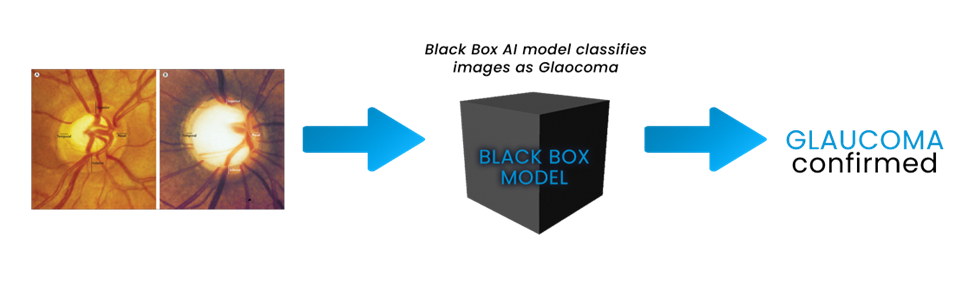
\includegraphics[scale=0.70]{images/fig-1.png}
\caption{Blackbox models confirming glaucoma through images}
\label{fig:x Blackbox models confirming glaucoma through images}
\end{figure}

\vspace{5mm}
In Figure 4.2 we will see how black boxes actually work with the help of lime.

\vspace{5mm}
\begin{figure}[htbp]
\centering
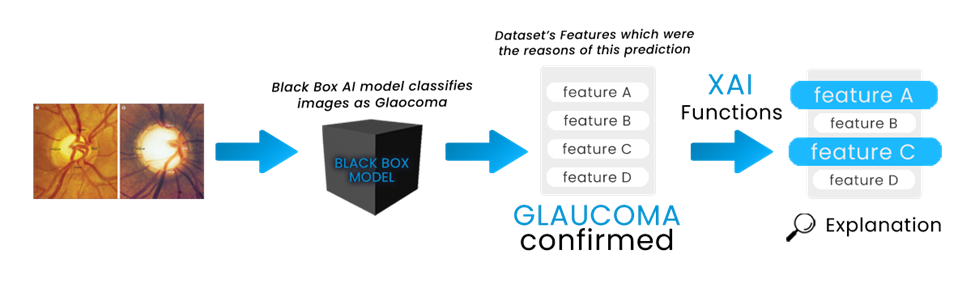
\includegraphics[scale=0.70]{images/fig-2.png}
\caption{Blackbox models decision making explanation through LIME}
\label{fig:x Blackbox models decision making explanation through LIME}
\end{figure}

\vspace{5mm}
\noindent Here we can see BlackBox models generate a result or output based on some features from the given/training datasets. And through lime, we can have a visualization from which features the output was based on.

\vspace{5mm}
\noindent In our Glaucoma dataset, we have some features for Suspicious glaucoma and Non-glaucoma. In both sections, we have fundus images, and labels as 1 as the confirmed glaucoma case and 0 as the Non-glaucoma case. To apply XAI, we took Fully Connected Neural Networks (FCNNs) as a black box AI model to predict glaucoma with the help of the data. To compile all of these classifications and determine the average of these scores to one single output, as in convolutional layers, we are using the ReLU nonlinear activation function and in the output nodes we are using the Softmax activation function. Below a short rendition is being given for the above Deep Learning models.

\vspace{5mm}
\noindent \textbf{1. Convolutional Neural Network (CNN)}: A convolutional neural network (CNN) is a type of deep neural network that is most typically used to evaluate visual images in deep learning. We will classify the image data through this model.

\vspace{5mm}
\noindent \textbf{2. Fully Connected Neural Network (FCNNs)}: FCNNs are a sort of artificial neural network in which all nodes, or neurons, in one layer are linked to neurons in the following layers [22]. FCNN model will also help us to predict and output.

\vspace{5mm}
\noindent \textbf{3. ReLU}: The activation function is implemented using a rectified linear activation unit, or ReLU for shorthand. Rectified networks are sometimes referred to as networks with hidden layers that employ this rectifier function. The computational cost of adding more ReLUs increases linearly as the size of the CNN grows.

\vspace{5mm}
\noindent \textbf{4. Softmax}:  that converts an integer vector into a probabilities vector, with the likelihood of each value proportional to the vector's relative scale is called softmax.  This model is programmed to generate N values, one for each classification task class, and the softmax function is used to normalize the outputs, converting these form weighted sum values to probabilities that add to just one. It is used for multi-classification in a logistic regression model, used in output layers for those networks that classify the inputs into multiple groups. This will compile all the convolutional layers of the FCNNs into a single output.

\newpage
\section{Work Plan} 
According to our Dataset, we will divide the data chronologically into training and testing data to classify glaucoma.. And through Lime, a XAI function, we will explain these black boxes.

\begin{figure}[htbp]
\centering
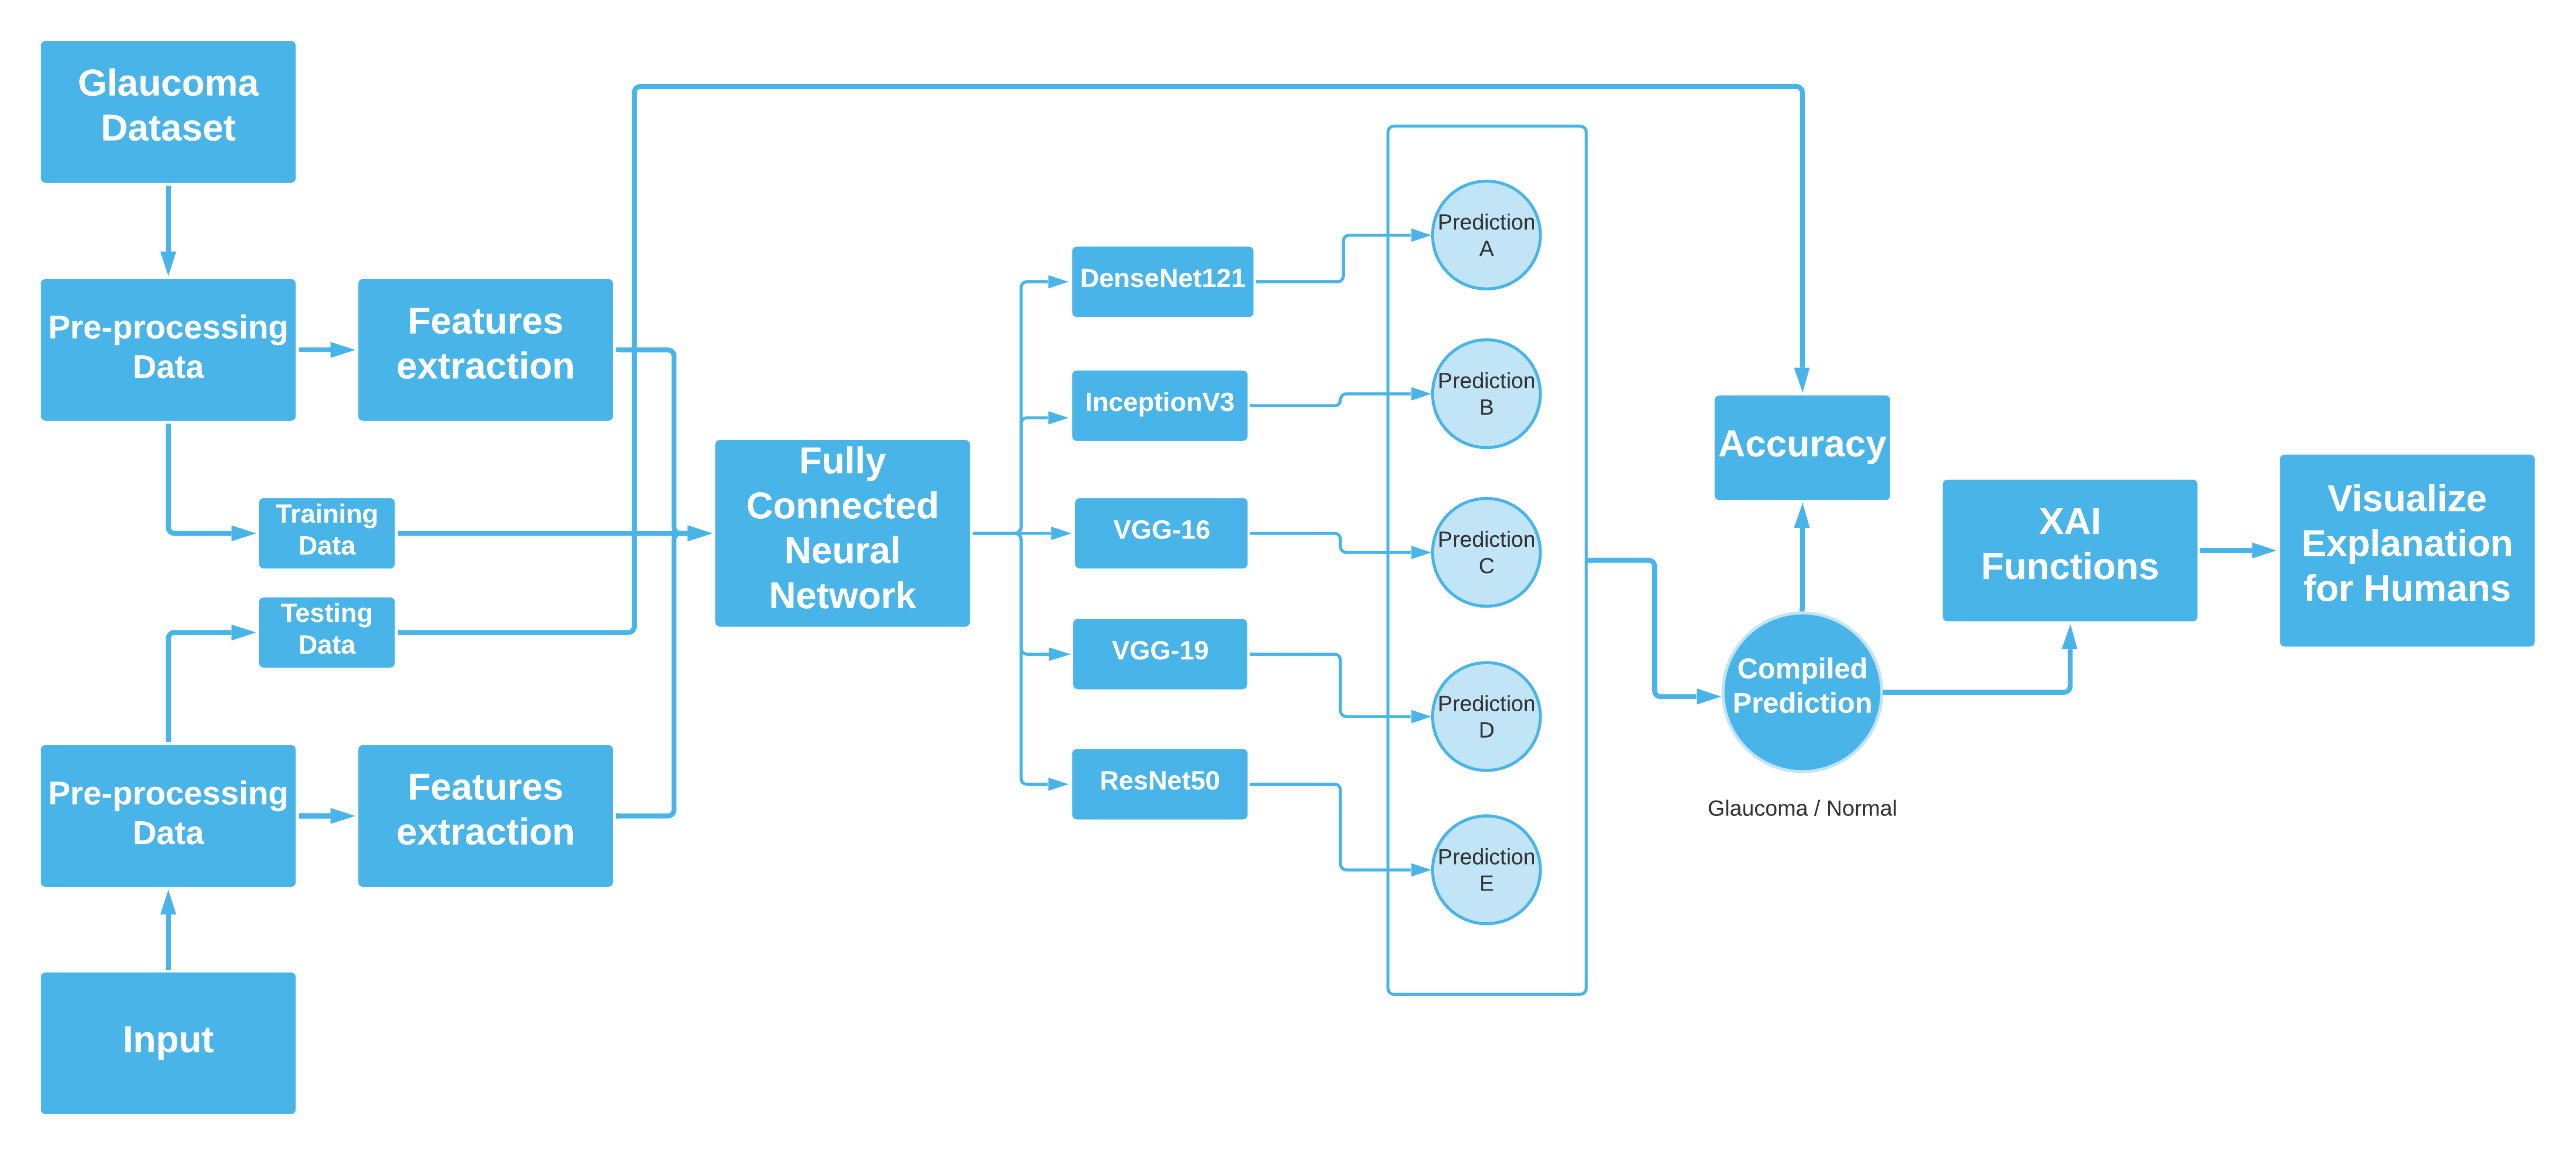
\includegraphics[scale=0.08]{images/work plan.png}
\caption{Work plan of the whole project}
\label{fig:x Work plan of the whole project}
\end{figure}

\vspace{5mm}
\noindent Here in [Figure 4.3], we have shown the whole process from dataset preprocessing to compiled output through Softmax activation function. And with XAI functions, we will explain the black boxes through visualization charts of the used core features which were the main reasons behind the prediction.

\vspace{5mm}
\noindent In our glaucoma dataset, we have some features for suspicious glaucoma and non-suspicious glaucoma. However, data visualization methods aim to produce more transparent and explainable decisions. In addition, CNN Based models are visually explainable for decision making and have gained significant attention in image classification [4]. A few works focus on preparing a Convolution Neural Network (CNN) by brute force while others use division and element extraction methods to identify glaucoma [5]. To apply for XAI we took Conventional Neural Network (CNN) architecture with fully connected layers or in other words Fully Connected Neural Network (FCNN). XAI frameworks LIME has been used for building trust among humans about the decisions made by AI models which are possibly making the black box models more transparent. Moreover, working with these AI models is not understandable by the common man and professionals. Additionally, AI and Machine Learning are essential for building trust among humans for decision making which is only possible by making black-box models more transparent through Explainable AI Frameworks which tries to explain their working.

\chapter{Implementation}
%\section{Implementation}
\section{Fundamentals of Deep Learning}

The manner in which people gain specific kinds of information, deep learning is that sort of AI and ML to impersonate. While conventional AI computation are straight, deep learning calculations are stacked in an order of expanding intricacy and deliberation. [23].
Neural Networks are basically made-up of several units which work mimicking the human brain’s neurons. Each neuron is connected to another one in order to generate a particular problem to solve. These neurons in AI are called units.
The input layer is the very first neuron of an Artificial brain. It takes raw data from the dataset and passes it to the next-level neurons. And the layer which produces the final output is called the output layer. N total of group may be composed by these input and output layers. Moreover, output layers’ units may depend on the output layer classes. In between these two layers, there can be N numbers of hidden layers, each containing its own weights and biases so that it can calculate its next neuron’s journey. The given density of the network is duplicated to its comparing info and afterward added up bringing about a weighted total, on which the initiation work suggests and delivers the actuation for that neuron, which is without a doubt the result of the neuron signified by y. Then, an activation function will get triggered as an output for this y.


\vspace{5mm}
\begin{figure}[hbt!]
\centering
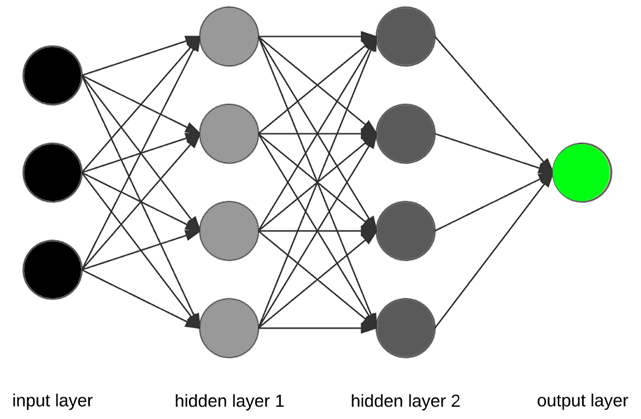
\includegraphics[scale=0.3]{images/fig-4.png}
\caption{Hidden Layer Between Input and Output Layers}
\label{fig:x Hidden Layer Between Input and Output Layers}
\end{figure}

\section{Dataset, Libraries, and Tools}
As our data are mostly direct fundus images from LAG-Dataset[24]. CNN is being used in this thesis for image classification, as it is a type of model which processes data such as images. Also, it automatically understands low-to high-level patterns of image classification. which helps us to extract higher representations for the image content.

\vspace{5mm}
\begin{figure}[htbp]
\centering
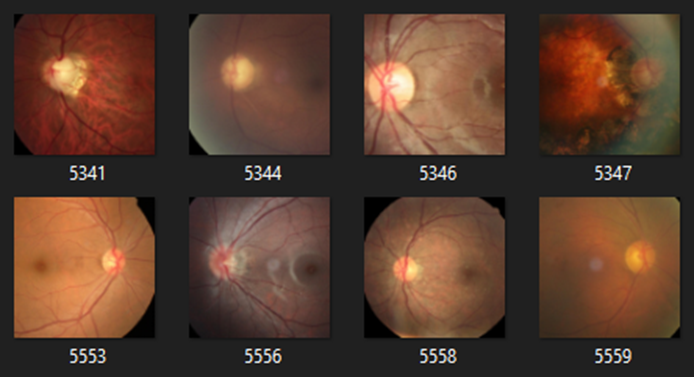
\includegraphics[scale=1]{images/fig-5.png}
\caption{Sample Data form LAG-Dataset}
\label{fig:x Sample Data form LAG-Dataset}
\end{figure}

\noindent This dataset contains 4250 images for \textbf{training}, 302 images for \textbf{testing} and 302 images for \textbf{validation}. All of these folders have two folders for glaucoma and non-glaucoma. The label for “glaucoma” is 1 and for “non-glaucoma” is 0.

\vspace{5mm}
\begin{table}[htbp]
\centering
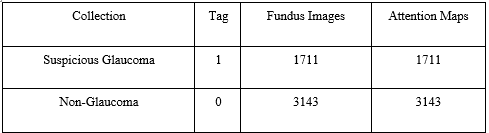
\includegraphics[scale=1]{images/fig_6.png}
\caption{\label{tab:Dissemination of data with tags}Dissemination of data with tags}

% \label{fig:x Dissemination of data with tags }
\end{table}

\noindent In this study, we are going to use the \textbf{python} for coding which is a high level Object Oriented Programming language that has a lot of amazing Machine learning libraries.

\vspace{5mm}
\noindent For this research we are using :

\begin{itemize}
    \item IDE (Google Colab & Jupyter Notebook)
    \item GPU (GTX 1660 super OC)
\end{itemize}

\newpage
\noindent Some of the Libraries that we are going to use are :

\vspace{5mm}
\noindent \textbf{TensorFlow}: TensorFlow is an endways open-source platform for AI that has a far reaching, adaptable biological system of instruments, libraries, and networks [17].

\vspace{5mm}
\noindent \textbf{Keras}: Keras is the prominent Programming interface of TensorFlow 2: a receptive, highly productive point of interaction for taking care of AI issues [18]

\vspace{5mm}
\noindent \textbf{Matplotlib}: Matplotlib is an extensive library for making fixed, energized, and intuitive representations in Python. [25]

\vspace{5mm}
\noindent \textbf{Pandas}: Pandas is an open-source, BSD-authorized library giving elite execution, simple to-utilize information designs, and information reasoning mechanism for Python programming [26]

\vspace{5mm}
\noindent \textbf{Numpy}: NumPy offers thorough numerical actions, random number generators, direct variable-based math schedules, Fourier changes, etc. [19]

\vspace{5mm}
\noindent \textbf{Scikit-Learning}: Straightforward and proficient devices for prescient information investigation Available to everyone, and reusable in different settings · Based on NumPy, SciPy, and matplotlib [27]

\section{Architecture of the Proposed Model}
A class of artificial neural structure which is most commonly enforced to analyze visual imagery is termed as deep learning or a convolutional neural network (CNN, or ConvNet) [20].

\vspace{5mm}
\noindent Transfer Learning approach is proposed in this study. Data set’s size and features provide a perfect environment for implementing a transfer learning approach, allowing a upskilled CNN with all of its density to be utilized to develop a new transfer learning model specialized to identifying Glaucoma with a high degree of accuracy.


\vspace{5mm}
\begin{figure}[hbt!]
\centering
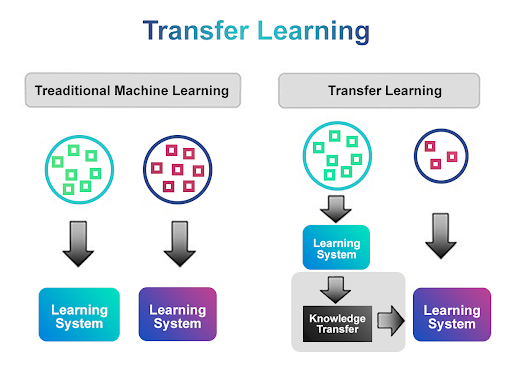
\includegraphics[scale=0.75]{images/fig-7.png}
\caption{Sample Data form LAG-Dataset}
\label{fig:x Sample Data form LAG-Dataset}
\end{figure}

\vspace{5mm}
\noindent We are going with the Fine-Tuning approach of Transfer Learning.

\vspace{5mm}
\noindent The CNN Models we are using are:

\begin{itemize}
    \item VGG-16
    \item InceptionV3
    \item VGG-19
    \item ResNet50
    \item DenseNet121
\end{itemize}

\subsection{VGG-16}
With 16-19 layers of density and little convolution strainers of (33), the VGG [29] Convolutional Neural Network worked by Visual Geometry Group, the University of Oxford has accomplished astounding outcomes. ReLU non-directly is utilized here for invisible layers.

\vspace{5mm}
\noindent In figure 5.4 we can visualize the planning of the VGG-16 model.


\vspace{5mm}
\begin{figure}[hbt!]
\centering
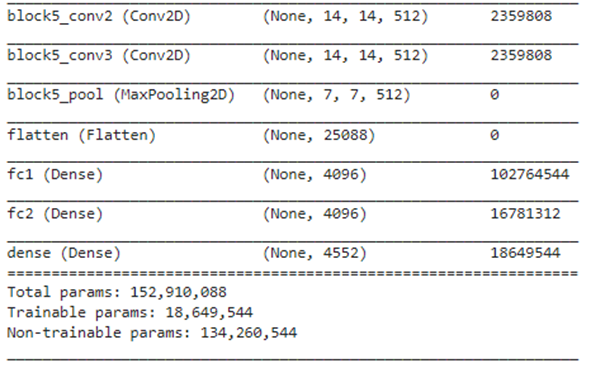
\includegraphics[scale=0.5]{images/fig-8.png}
\caption{Proposed Summary of VGG-16}
\label{fig:x Proposed Summary of VGG-16}
\end{figure}

\vspace{5mm}
\noindent Here we used Keras implementation of VGG-16 model. We used the weights learned from the ImageNet dataset. After downloading the pre-trained model we have made every trained layers into untrainable layers and deleted the top 3 layer layers to reuse the model. Then we use a Flatten layer to flatten every previous models layers into one and we used 3 Dense neurons with 100 layers in each of them. Input shape of our dataset's images are 224 x 224. We used the “ReLU” activation function for the Convolutional layers. For predictions, we used the A Dense neuron with 2 layers in it for 2 output (Glaucoma and Non-glaucoma) and “Softmax” for activation function.

\vspace{5mm}
\noindent In figure 5.5 we can visualize the architecture of the VGG-16  model.

\vspace{5mm}
\begin{figure}[hbt!]
\centering
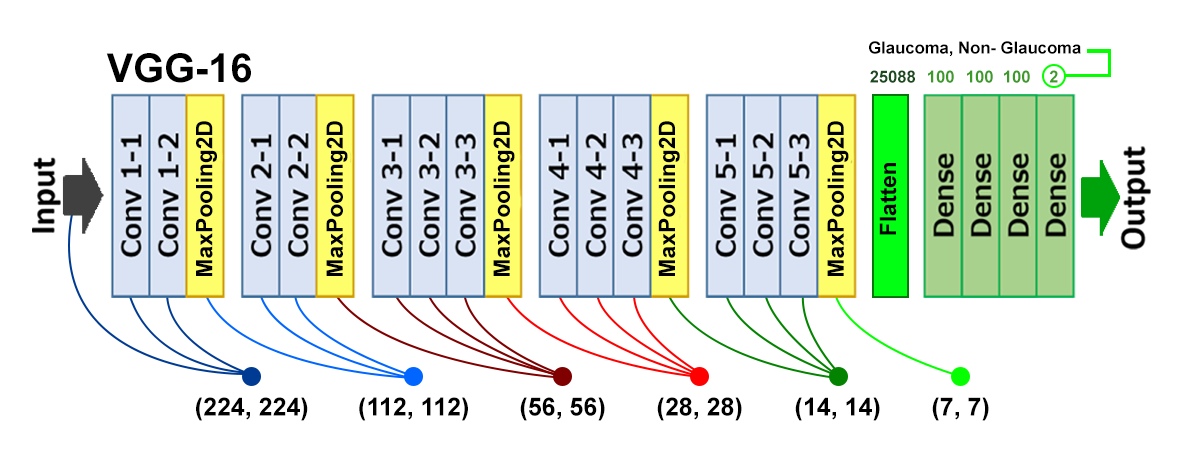
\includegraphics[scale=0.75]{images/Architecture of VGG-16.png}
\caption{Architecture of VGG-16}
\label{fig:x Architecture of VGG-16}
\end{figure}

\subsection{Inception V3}
The Inception [30] architecture is made up of several inception modules stacked on top of each other to form a deep neural network, where the inception modules provide the ability to work them all in equal and link their results into a solitary result vector for contribution to the module a short time later.

\vspace{5mm}
\noindent In figure 5.6 we can visualize our model summary of InceptionV3.

\vspace{5mm}
\begin{figure}[hbt!]
\centering
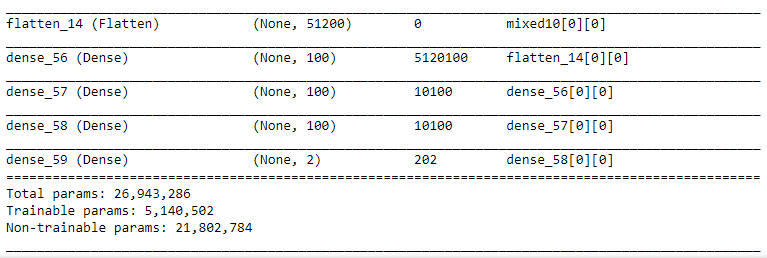
\includegraphics[scale=0.75]{images/fig-11.png}
\caption{Model Summary of InceptionV3}
\label{fig:x Model Summary of InceptionV3}
\end{figure}

\vspace{5mm}
\noindent Here we used Keras implementation of InceptionV3 model. We used the weights learned from the ImageNet dataset. After downloading the pre-trained model we have made every trained layers into untrainable layers and deleted the top 3 layer layers to reuse the model. Then we use a Flatten layer to flatten every previous models layers into one and we used 3 Dense neurons with 100 layers in each of them. Input shape of our dataset's images are 224 x 224. We used the “ReLU” activation function for the Convolutional layers. For predictions, we used the A Dense neuron with 2 layers in it and “Softmax” for activation function.

\subsection{VGG-19}
VGG19 is a variation of the VGG model which in short comprises of 19 layers (16 convolution layers, 3 completely associated layers, 5 MaxPool layers, and 1 SoftMax layer). [32] VGG19 has 19.6 billion Failures. In Figure 5.7, Our model summary for VGG-19 is given.

\vspace{5mm}
\begin{figure}[hbt!]
\centering
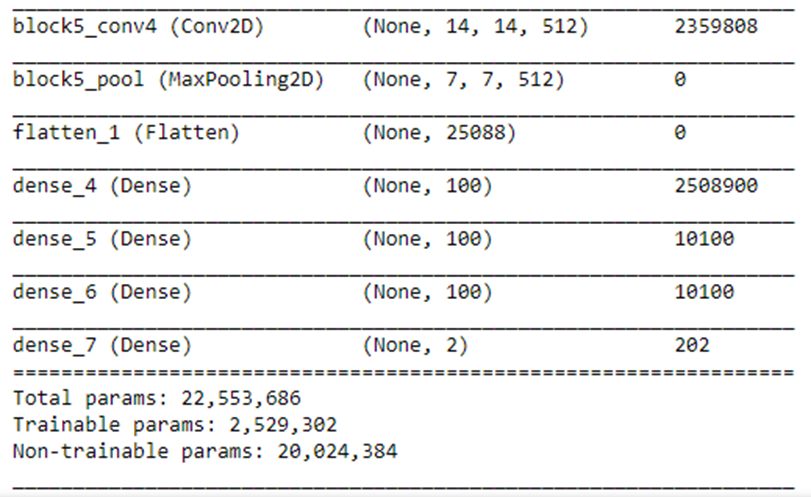
\includegraphics[scale=1]{images/fig-12.png}
\caption{Model Summary of VGG-19}
\label{fig:x Model Summary of VGG-19}
\end{figure}

\vspace{5mm}
\noindent Here we used Keras implementation of VGG-19 model. We used the weights learned from the ImageNet dataset. After downloading the pre-trained model we have made every trained layers into untrainable layers and deleted the top 3 layer layers to reuse the model. Then we use a Flatten layer to flatten every previous models layers into one and we used 3 Dense neurons with 100 layers in each of them. Input shape of our dataset's images are 224 x 224. We used the “ReLU” activation function for the Convolutional layers. Then we performed batch normalization used a dropout rate of 0.5. In Figure 5.8, Our model summary for VGG-19 is given.

\vspace{5mm}
\begin{figure}[hbt!]
\centering
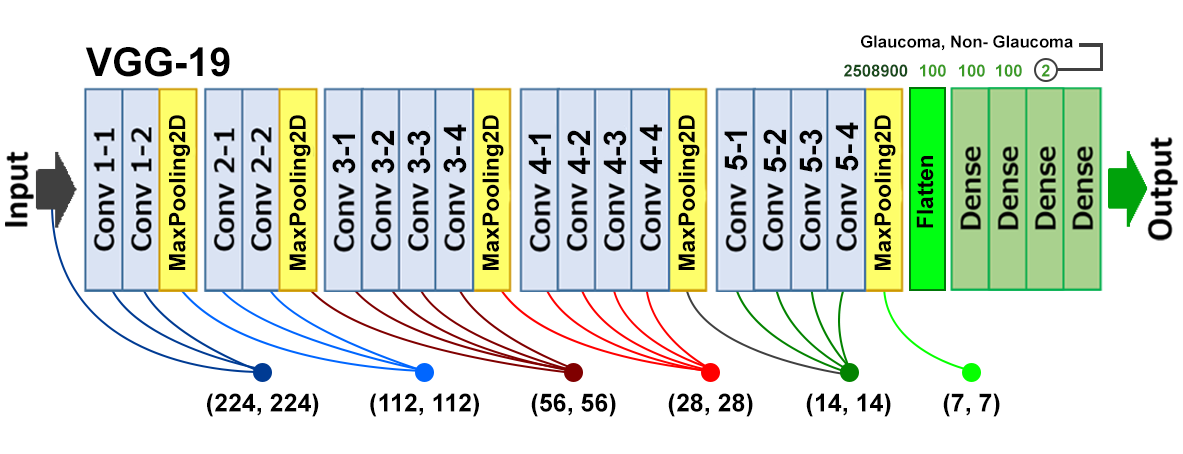
\includegraphics[scale=0.75]{images/Architecture of VGG-19.png}
\caption{Architecture of VGG-19}
\label{fig:x Architecture of VGG-19}
\end{figure}

\vspace{5mm}
\noindent For expectations, we involved the A Thick neuron with 2 layers in it and "Softmax" for initiation work. For the Angle Drop, we utilized the Adam enhancer with a learning pace of \(10^-5\).

\subsection{ResNet50}
ResNet50 is a variant of the ResNet model which has 48 convolution layers and 1 MaxPool layer and 1 normal pool layer. Besides, it has 3.8 x 109 floating point activities. ResNet50 assumes a significant part in the computer vision and profound learning world. It is principally utilized for picture acknowledgment and is most ordinarily applied for dissecting visual symbolism. Additionally, it is a pre-prepared Profound Learning model for picture order of the Convolutional Neural Organization (CNN).  ResNet50 is mainly trained on a million images of 1000 categories from the ImageNet database and there are over 23 million trained parameters which will make it more suitable for image recognition. ResNet50 is deeper than any other network using residual connections. In Figure 5.9, we can visualize the architecture of a ResNet50 model.

\vspace{5mm}
\noindent In Figure 5.9, we can visualize the architecture of a ResNet50 model.

\vspace{5mm}
\begin{figure}[hbt!]
\centering
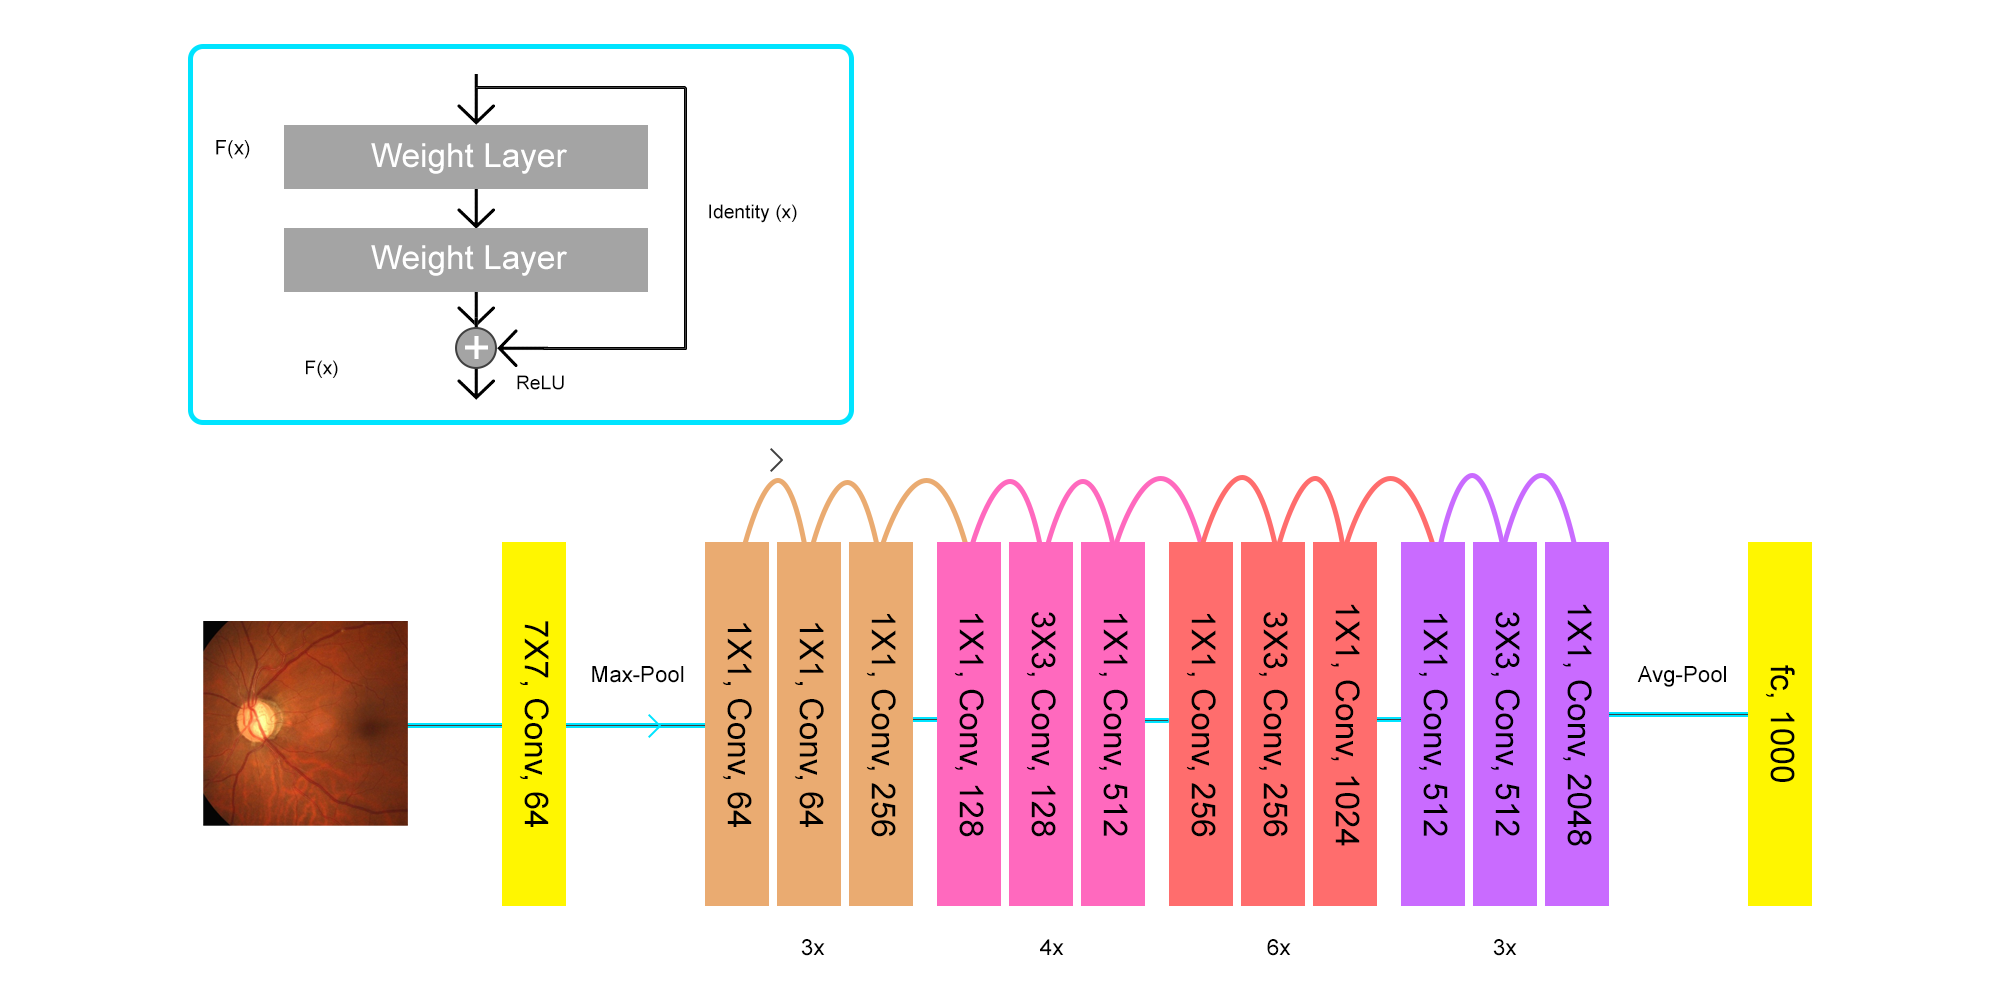
\includegraphics[scale=0.45]{images/resnet50.png}
\caption{Architecture of ResNet50}
\label{fig:x Model Summary of ResNet50}
\end{figure}

\vspace{5mm}
\begin{figure}[hbt!]
\centering
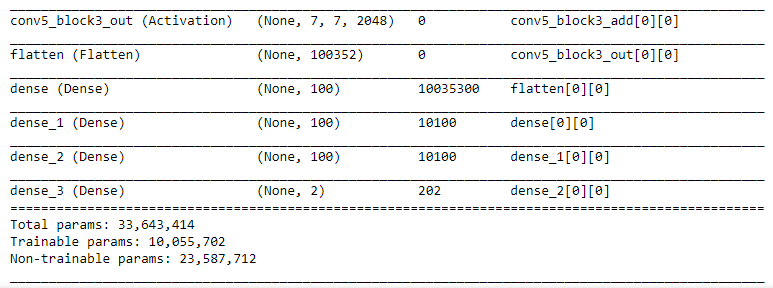
\includegraphics[scale=0.7]{images/ResNet50.PNG}
\caption{Model Summary of ResNet50}
\label{fig:x Model Summary of ResNet50}
\end{figure}

\vspace{5mm}
\noindent Here, we used the Keras implementation of the ResNet50 Model. We used the weights learned from the ImageNet dataset. After downloading the pre-trained model we have made every trained layers into untrainable layers and deleted the top 3 layer layers to reuse the model. Then we use a Flatten layer to flatten every previous models layers into one and we used 3 Dense neurons with 100 layers in each of them. Input shape of our dataset's images are 224 x 224. We used the “ReLU” activation function for the Convolutional layers. For predictions, we used the A Dense neuron with 2 layers in it and “Softmax” for activation function. 



\subsection{DenseNet121}
Dense Convolutional Network which is DenseNet is a design that bright lights on making the significant learning networks go impressively more significant, but making them more capable to get ready, by using more restricted relationship between the layers [33]. DenseNet is actually similar to ResNet for specific key differentiations. For example, ResNet uses an additional substance system that consolidates the former layer with the future layer, while DenseNet joins the consequence of the first layer with the future layer. This is done to enable the best information stream between the layers of the association.

\vspace{5mm}
\begin{figure}[hbt!]
\centering
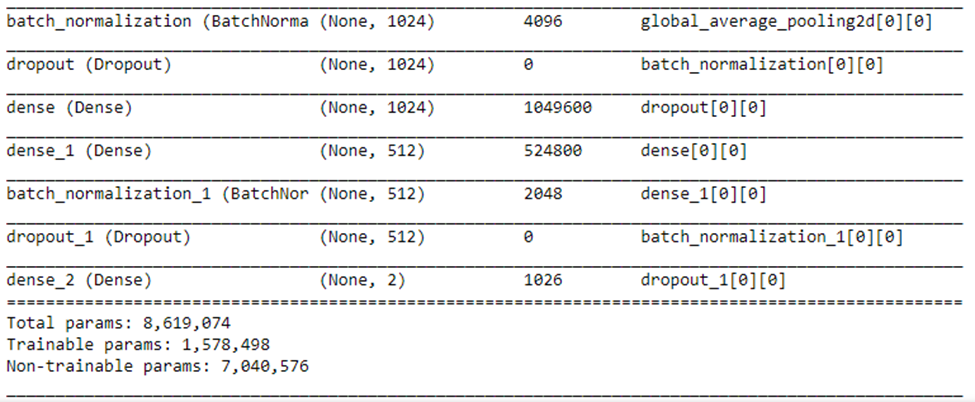
\includegraphics[scale=0.5]{images/fig-15.png}
\caption{Model Summary of DenseNet121}
\label{fig:x Model Summary of DenseNet121}
\end{figure}
\vspace{5mm}

\vspace{5mm}
\begin{figure}[hbt!]
\centering
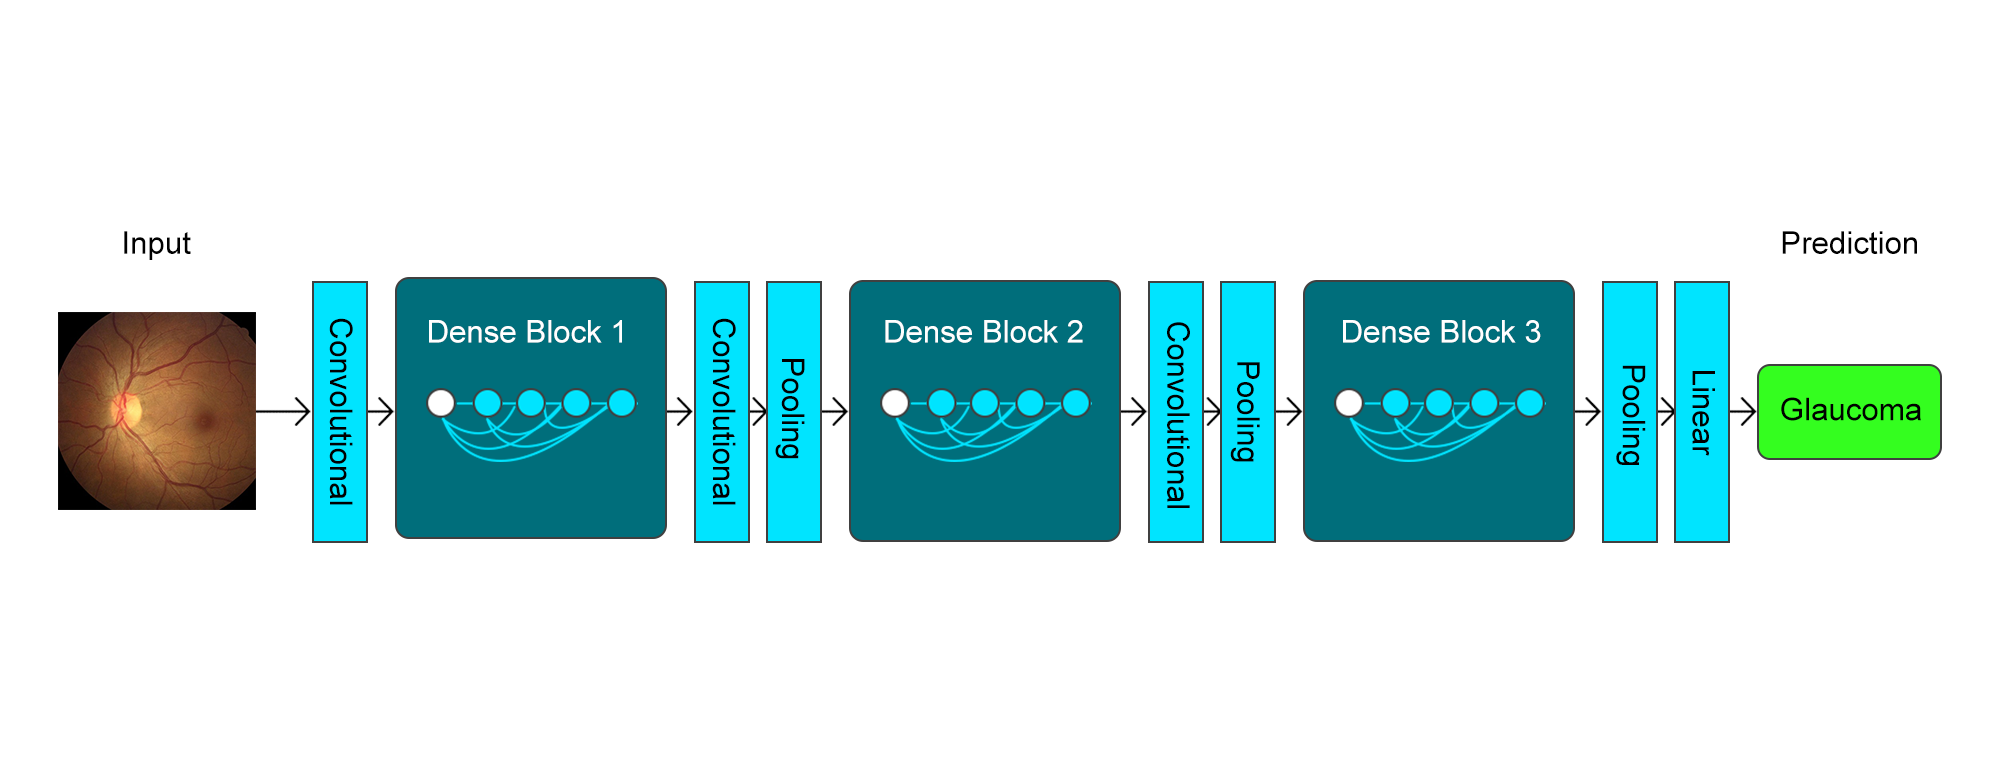
\includegraphics[scale=0.4]{images/densenet archinew.png}
\caption{Architecture of DenseNet121}
\label{fig:x Model Summary of DenseNet121}
\end{figure}
\vspace{5mm}

\noindent Here, we used the Keras implementation of the DenseNet121 model . We used the weights learned from the ImageNet dataset. After downloading the pre-trained model we have made every trained layers into untrainable layers and deleted the top 3 layer layers to reuse the model. Then we use a Flatten layer to flatten every previous models layers into one and we used 3 Dense neurons with 1024 layers, 512 layers and 256 layers in each of them. Input shape of our dataset's images are 224 x 224. We used the “ReLU” activation function for the Convolutional layers. For predictions, we used the A Dense neuron with 2 layers in it and “Softmax” for activation function.



\section{Fine Turing}
Fine-tuning is the process of fine-tuning or changing a model which has previously been trained for one job to make it work as a 2nd task which was related. A deep learning network that recognizes cars, for example, maybe fine-tuned to recognize trucks [25]. As proposed, we will be using Fine-tuning approach to detect Glaucoma from our dataset which will help to detect our wanted result in this study.

\vspace{5mm}
\begin{figure}[hbt!]
\centering
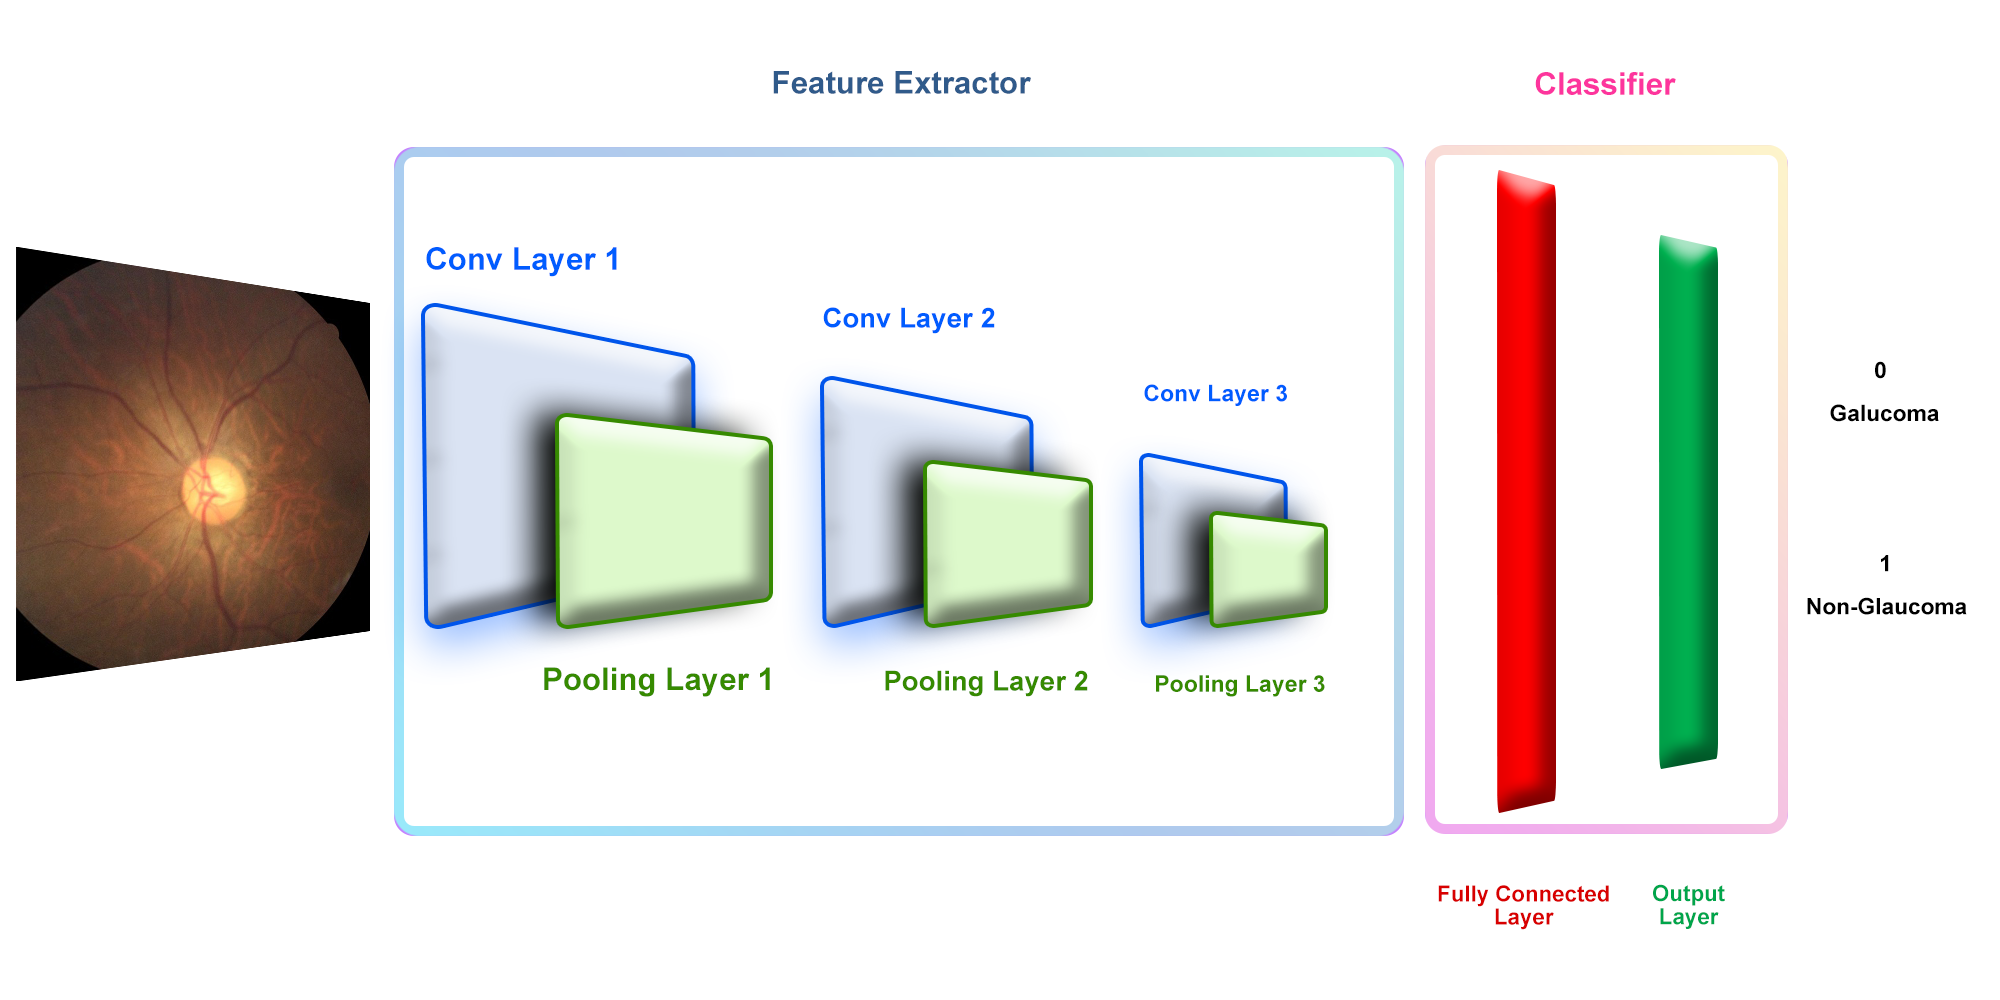
\includegraphics[scale=0.4]{images/Fine-tuning by keeping the feature extractor_s final layers trainable.png}
\caption{Fine-tuning by keeping the feature extractor's final layers trainable}
\label{fig:x Fine-tuning by keeping the feature extractor's final layers trainable}
\end{figure}

\newpage
\subsection{Segments of CNN}

\vspace{5mm}
The architecture of Convolutional Neural Networks is basically 3 types of layers.

\begin{itemize}
    \item Convolutional
    \item Pooling
    \item Fully Connected
\end{itemize}

\vspace{5mm}
\begin{figure}[hbt!]
\centering
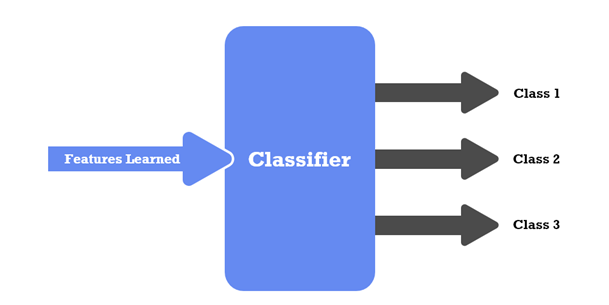
\includegraphics[scale=1]{images/fig-17.png}
\caption{CNN Classifier}
\label{fig:x CNN Classifier}
\end{figure}

\noindent And basically, all these layers do these operations as bellow:

\vspace{5mm}
\begin{itemize}
    \item Convolution operation
    \item Pooling operation
    \item Flattening
    \item Non-linear activation functions imply
    \item Optimization operation
\end{itemize}

\vspace{5mm}
\subsection{Convolutional Operation}


\vspace{5mm}
As illustrated in \textbf{figure 5.15}, the convolutional layers are responsible for convolution operations and create feature maps that learn the characteristics of the image taken as input by convolving correctly learnt filters or kernels with the input array or tensor. \textbf{Figure 5.16} shows how a convolution operation contains a number of feature maps that record new features and respond to feature hierarchy across the neural network, from the early layers to the far edging layers. [29] [34] [30]

\vspace{5mm}
\begin{figure}[hbt!]
\centering
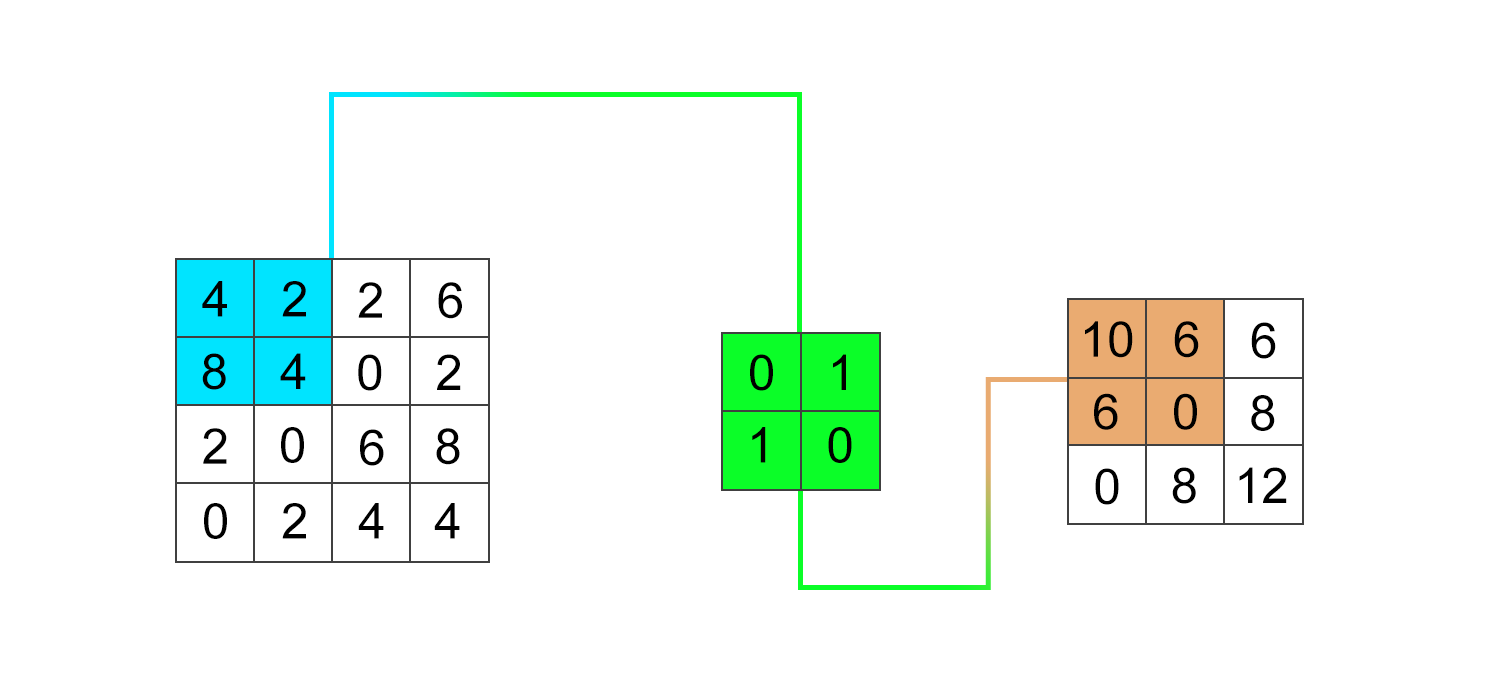
\includegraphics[scale=0.5]{images/feature map.png}
\caption{Convolution Operation}
\label{fig:x Convolution Operation}
\end{figure}

\vspace{5mm}
\begin{figure}[hbt!]
\centering
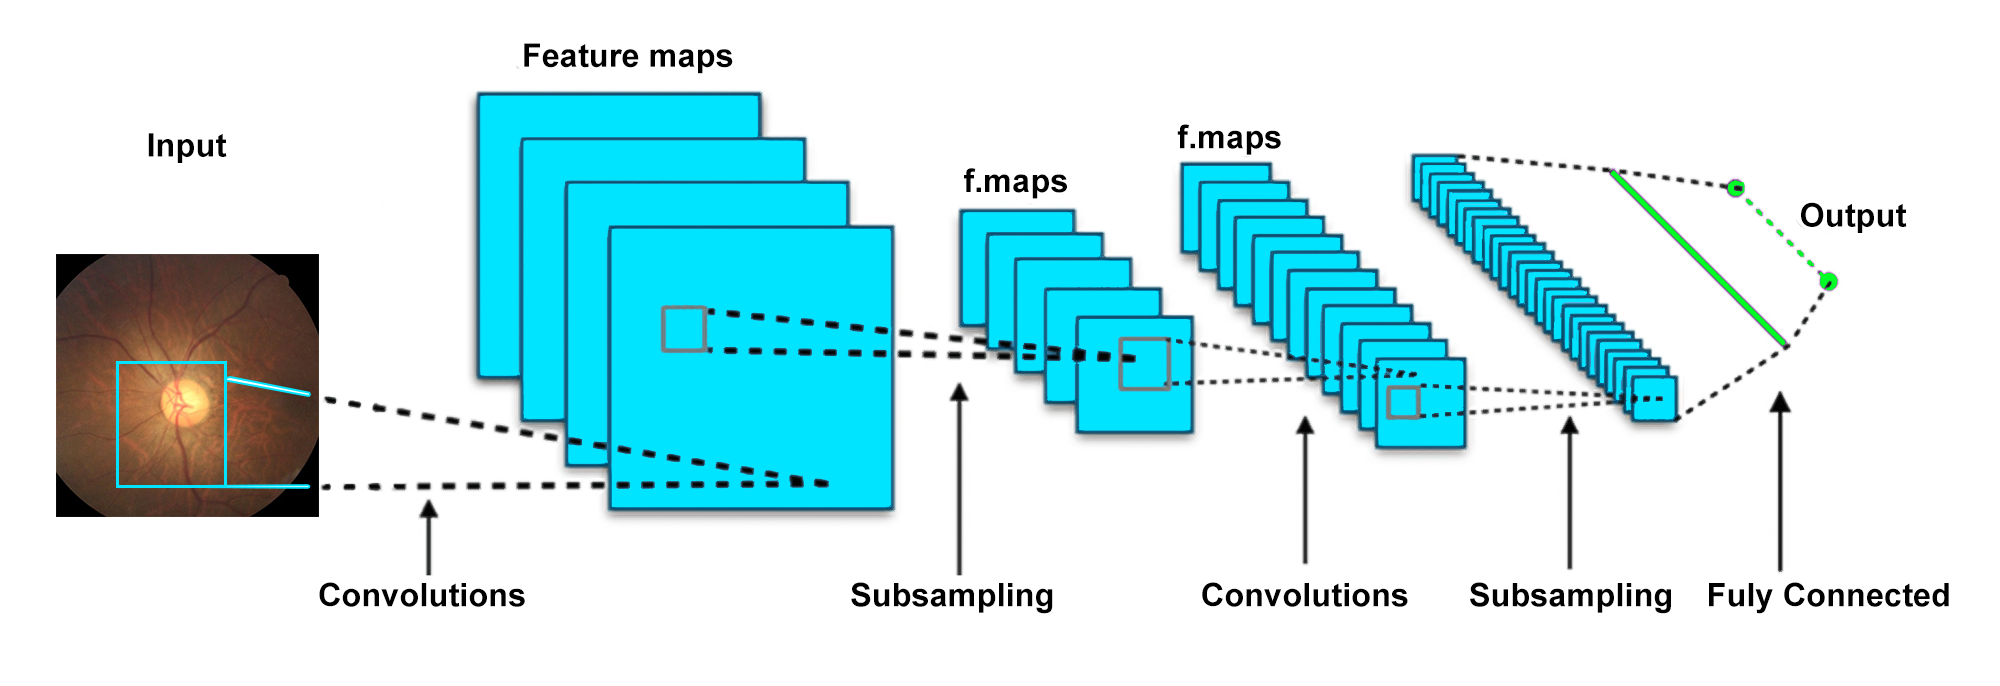
\includegraphics[scale=0.4]{images/planes shown are a feature map.png}
\caption{Feature map}
\label{fig:x Feature map}
\end{figure}

\newpage
\subsection{Pooling Operation}

\vspace{5mm}
The feature maps are pooled in order to extract more features and minimize their dimension[30]. In general, the pooling operation is carried out as follows:
\vspace{5mm}
\begin{figure}[hbt!]
\centering
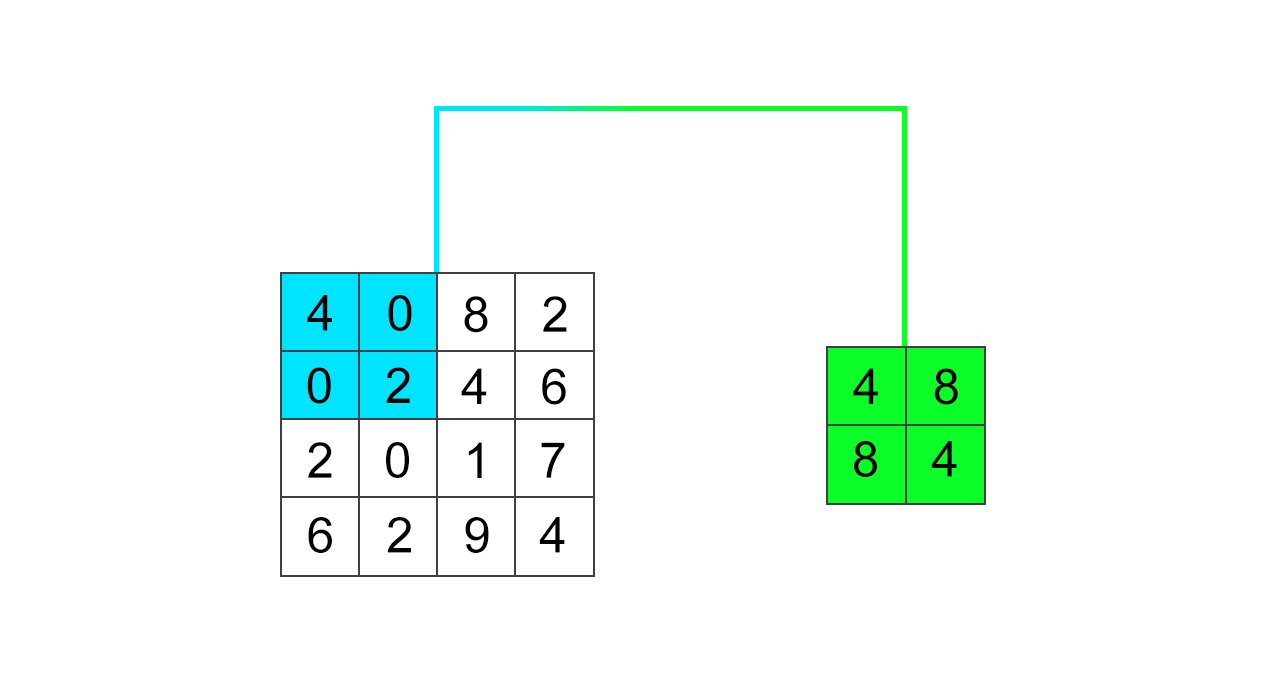
\includegraphics[scale=0.5]{images/pooling.png}
\caption{Pooling Operation}
\label{fig:x Pooling Operation}
\end{figure}
\vspace{5mm}
\begin{itemize}
    \item \textbf{Max Pooling}: As an output, the greatest value of a patch of numbers from the feature map that was utilized as input is returned. [30]
    \item \textbf{Average Pooling}: It produces the average as an output, the value of the patch of digits from the feature map that's been utilized as an input. [34]
    \item \textbf{GlobalAveragePooling2D}: GlobalAveragePooling2D takes a new approach. The spatial dimensions are average pooled until each spatial dimension is one.
\end{itemize}

\vspace{5mm}
\begin{figure}[hbt!]
\centering
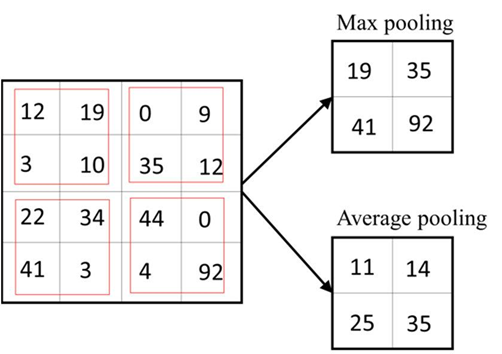
\includegraphics[scale=1]{images/fig-21.png}
\caption{Max and Average Pooling}
\label{fig:x Max and Average Pooling}
\end{figure}

\vspace{5mm}
\subsection{Flattening Layers}

\vspace{5mm}
The process of flattening data into a one-dimensional array for usage in the next layer is known as flattening. To produce a single lengthy feature vector, we flatten the output of a convolutional layers. It's also related to the final categorization model, as a fully-connected layer [35].

\vspace{5mm}
\begin{figure}[hbt!]
\centering
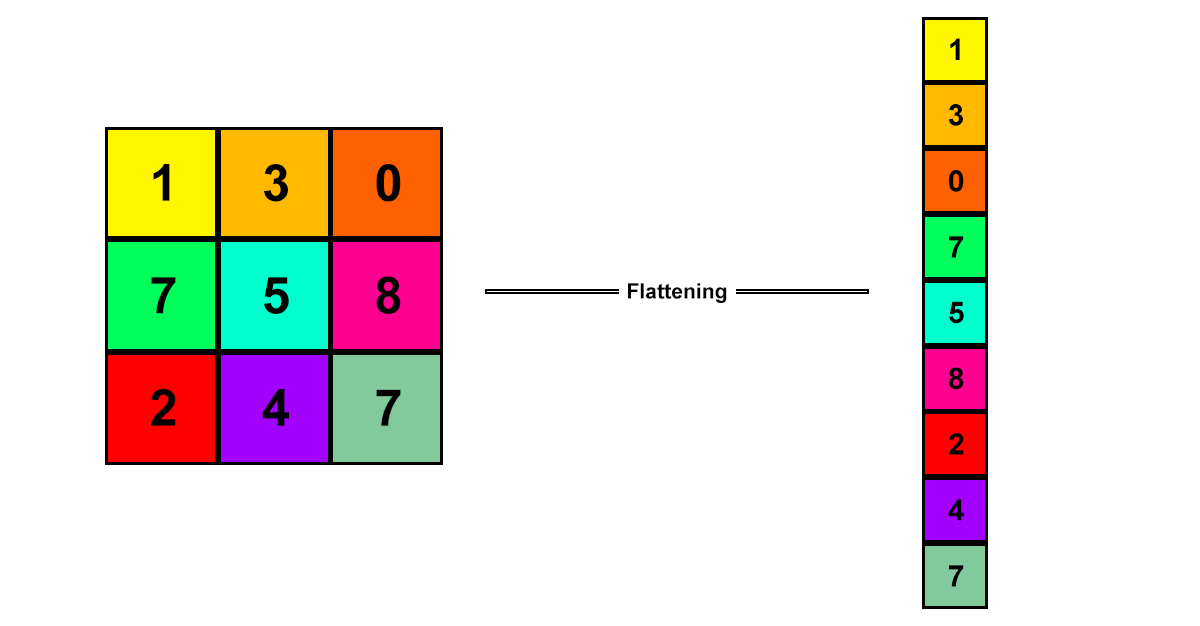
\includegraphics[scale=0.5]{images/Pooling Matrix to Flattening..png}
\caption{Pooling Matrix to Flattening.}
\label{fig:x Pooling Matrix to Flattening}
\end{figure}

\vspace{5mm}
\subsection{Fully Connected Layers}

\vspace{5mm}
Fully linked layers in a neural network are those where all of the inputs through one layer are connected with every activation unit of next layer. In most common machine learning models, these last several layers are fully linked layers that combine the data acquired by previous levels to generate the final output [36].

\vspace{5mm}
\begin{figure}[hbt!]
\centering
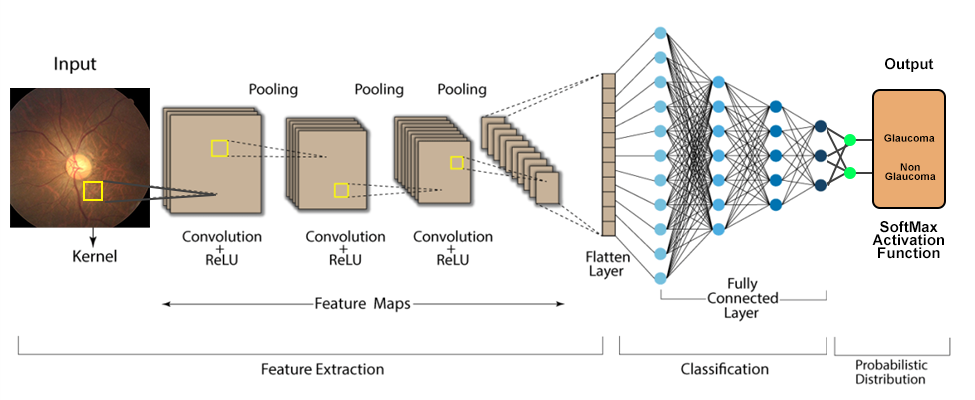
\includegraphics[scale=0.45]{images/Fully Connected CNN classifying between classes.png}
\caption{Classifying different classes using a fully connected CNN}
\label{fig:x Classifying different classes using a fully connected CNN}
\end{figure}

\noindent Fully connected layers or in other words dense layers take nonlinear activation functions, however, the final output layer of the fully connected layers take Softmax activation.

\vspace{5mm}
\noindent We are also going to use SoftMax and ReLU in both VGG-16 and InceptionV3.

\vspace{5mm}
\subsection{Optimization Algorithm}
\vspace{5mm}
\noindent When deep learning is utilized for training, an optimization technique is applied to improve the cost function. This algorithm's general equation is as follows:

\vspace{5mm}
\begin{equation*}
J(W,\ b) = \frac{1}{m}\sum_{i=1}^m\ L(y^{'i},y^i)
\end{equation*}

\vspace{5mm}
\noindent We applied Adam optimizer in our models, which would be discussed below: Algorithm Adam is a well-known algorithm that is noted for the speed it contains. Adaptive Momentum is the abbreviation for AdaM. At the same time, Adam associates the propulsion RMSprop. As a result, Adam is a highly powerful and quick algorithm. This approach is relatively straightforward in its implementation, quite efficient in estimate, and uses very little memory. For larger issues with data or parameters, it is more efficient. The optimizer is defined by the equations below:

\vspace{5mm}
\begin{equation*}
\begin{split}
\alpha_t = \alpha.\frac{\sqrt{1-\beta^t_2}}{1-\beta^t_2} \\
\theta_t\leftarrow\theta_{t-1}-\alpha_t-.m_{\frac{t}{(\sqrt{v_t}+\hat{\epsilon})}}
\end{split}
\end{equation*}
\vspace{5mm}
For the Gradient Descent, we used the Adam optimizer with a learning rate of 10-5. 

\vspace{5mm}
\subsection{Softmax}
\vspace{5mm}
\noindent The output of this function is a probability distribution. As the entire summation becomes 1, it maps the input. This function is defined by the equation given below:

\vspace{5mm}
\begin{equation*}
f_j(z)=\frac{e^{zj}}{\sum_k{e^zk}} 
\end{equation*}

\vspace{5mm}
\noindent It squashes a vector of arbitrary real-valued scores (in z) into a vector of values between 0 and 1 that add to 1.

\vspace{5mm}
\subsection{Rectified Linear Unit (ReLU)}
\vspace{5mm}
\noindent ReLU is a piecewise linear function that directly outputs the input. It has a 0 to range. In the deep learning era, amongst most well-known activation function ReLU is the one, as seen in below mentioned equation:

\vspace{5mm}
\begin{equation*}
y=max(0,x) 
\end{equation*}

\vspace{5mm}
\noindent ReLU's main advantage is that it solves the vanishing gradient problem, is one-sided (unlike TanH), has sparse activation (50\%) and no back propagation error. This function is monotonic, as are its derivatives. the fact that this function is non-zero centered and non-differentiable by zero is a drawback. Another drawback is the dwindling ReLU population. which occurs when half of the outputs for non-zero centered action are inactive (returned as 0).


\vspace{5mm}
\subsection{Batch Normalization}

\vspace{5mm}
While feeding input to Neural Networks, we do Batch Normalization because it makes the training faster and handles internal covariate shift. Again Normalizing the input for a similar range of values can speed up the learning. Because Batch Normalization normalizes the outputs of the activation functions in every layer of the neural network, not just in the inputs. In their original paper, Sergey et al. [37] claim that it minimizes the network's inner covariate shift. 

\vspace{5mm}
\subsection{Dropout}

\vspace{5mm}
Adulteration of training information misleadingly regulates to over fit through dropout and other characteristically noise systems. Dropout holds out a kind of versatile regularization for summed up straight models [38]. Moreover, Dropout is a normal stochastic choice strategy in view of the neural organization [39]. It causes this level to appear and be handled as a level with a certain measure of hubs and availability in comparison to the previous level. Essentially, a particular perspective on the designed layer is directed with each update to a layer during preparing.

\newpage
\section{Analysis}
We have used VGG-16, VGG-19, DenseNet121, InceptionV3 and ResNet50 models for our study. Every model was compiled with Adam optimizer with the learning rate of 1e-5 in 50 epochs. 

\vspace{5mm}
\noindent After 50 epochs, RestNet50 got the highest score among the other models with a validation accuracy of 94.7\%.

\vspace{5mm}
\noindent These are the Train and Test score of our models - 

\begin{table}[hbt!]
\resizebox{\textwidth}{!}{%
\begin{tabular}{@{}|c|c|c|c|c|c|c|@{}}
\toprule
Model       & \multicolumn{1}{l|}{Epochs} & Accuracy & Train Accuracy & Train Loss & Validation Loss & \multicolumn{1}{l|}{Weight} \\ \midrule
DenseNet121 & \multirow{5}{*}{50}         & 86.81\%  & 88.83\%        & 31.18\%    & 24.10\%         & \multirow{5}{*}{ImageNet}   \\ \cmidrule(r){1-1} \cmidrule(lr){3-6}
InceptionV3 &  & 86.42\% & 93.49\% & 20.04\% & 35.79\% &  \\ \cmidrule(r){1-1} \cmidrule(lr){3-6}
ResNet50    &  & 94.71\% & 99.56\% & 3.81\%  & 12.22\% &  \\ \cmidrule(r){1-1} \cmidrule(lr){3-6}
VGG-16      &  & 88.63\% & 98.00\% & 6.76\%  & 27.92\% &  \\ \cmidrule(r){1-1} \cmidrule(lr){3-6}
VGG-19      &  & 93.31\% & 97.00\% & 11.53   & 14.94\% &  \\ \bottomrule
\end{tabular}%
}
\caption{Model Accuracy and Loss}
\label{tab:Model Accuracy and Loss}
\end{table}

\vspace{5mm}
\noindent Below the Train and Test accuracy and loss graph for each model are given.
\newpage
\vspace{5mm}
\noindent Model Accuracy and Loss of VGG-16 -

\vspace{5mm}
\begin{figure}[hbt!]
\centering
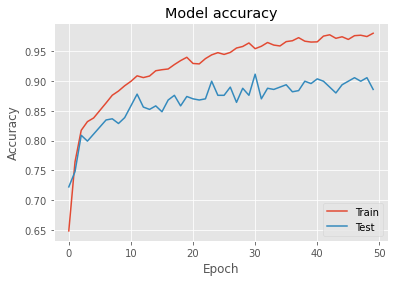
\includegraphics[scale=1]{images/fig-25.png}
\caption{VGG-16 Model Train and Test Accuracy}
\label{fig:x VGG-16 Model Train and Test Accuracy}
\end{figure}

\vspace{5mm}
\begin{figure}[hbt!]
\centering
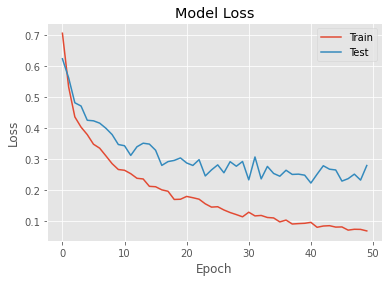
\includegraphics[scale=1]{images/fig-26.png}
\caption{VGG-16 Model Train and Test Loss}
\label{fig:x VGG-16 Model Train and Test Loss}
\end{figure}

\newpage
\noindent Model Accuracy and Loss of VGG-19 -

\vspace{5mm}
\begin{figure}[hbt!]
\centering
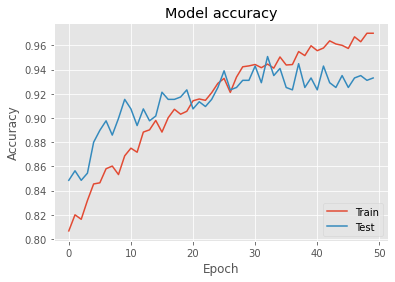
\includegraphics[scale=1]{images/fig-27.png}
\caption{VGG-19 Model Train and Test Accuracy}
\label{fig:x VGG-19 Model Train and Test Accuracy}
\end{figure}

\vspace{5mm}
\begin{figure}[hbt!]
\centering
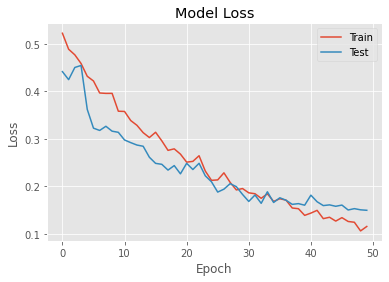
\includegraphics[scale=1]{images/fig-28.png}
\caption{VGG-19 Model Train and Test Loss}
\label{fig:x VGG-19 Model Train and Test Loss}
\end{figure}

\newpage
\vspace{5mm}
\noindent Model Accuracy and Loss of ResNet50 -
\vspace{5mm}
\begin{figure}[hbt!]
\centering
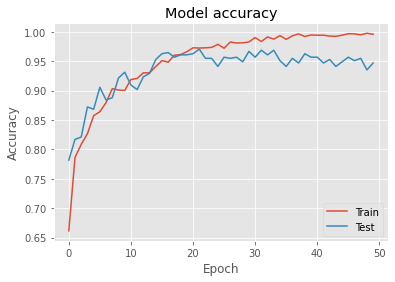
\includegraphics[scale=1]{images/fig-29.png}
\caption{ResNet50 Model Train and Test Accuracy}
\label{fig:x ResNet50 Model Train and Test Accuracy}
\end{figure}

\vspace{5mm}
\begin{figure}[hbt!]
\centering
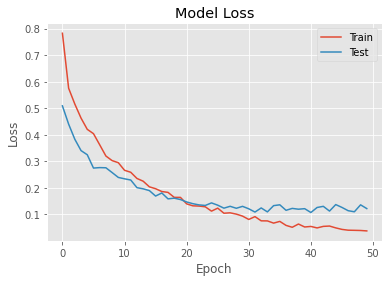
\includegraphics[scale=1]{images/fig-30.png}
\caption{ResNet50 Model Train and Test Loss}
\label{fig:x ResNet50 Model Train and Test Loss}
\end{figure}

\newpage
\vspace{5mm}
\noindent Model Accuracy and Loss of DenseNet121 -
\vspace{5mm}
\begin{figure}[hbt!]
\centering
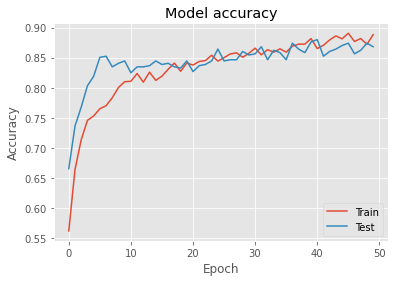
\includegraphics[scale=1]{images/fig-31.png}
\caption{DenseNet121 Model Train and Test Accuracy}
\label{fig:x DenseNet121 Model Train and Test Accuracy}
\end{figure}

\vspace{5mm}
\begin{figure}[hbt!]
\centering
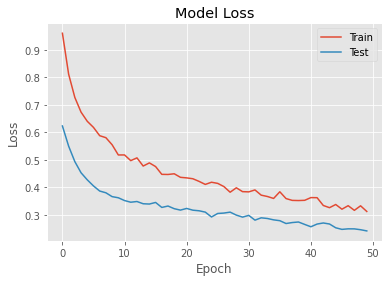
\includegraphics[scale=1]{images/fig-32.png}
\caption{DenseNet121 Model Train and Test Loss}
\label{fig:x DenseNet121 Model Train and Test Loss}
\end{figure}

\newpage
\vspace{5mm}
\noindent Model Accuracy and Loss of InceptionV3 -
\vspace{5mm}
\begin{figure}[hbt!]
\centering
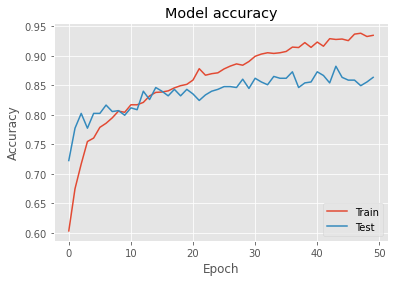
\includegraphics[scale=1]{images/fig-33.png}
\caption{InceptionV3 Model Train and Test Accuracy}
\label{fig:x InceptionV3 Model Train and Test Accuracy}
\end{figure}

\vspace{5mm}
\begin{figure}[hbt!]
\centering
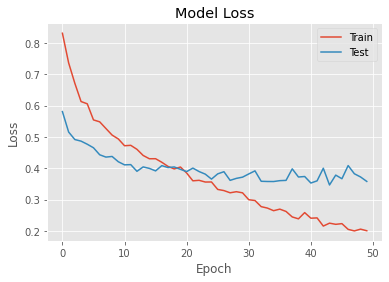
\includegraphics[scale=1]{images/fig-34.png}
\caption{InceptionV3 Model Train and Test Loss}
\label{fig:x InceptionV3 Model Train and Test Loss}
\end{figure}

\noindent The form and behavior of a learning curve may be used to analyze a machine learning model's performance, also advise what sort of config modifications should be required to enhance the production.

\vspace{5mm}
\noindent In learning curves, there are three main dynamics that you'll see. They are as follows:


\begin{itemize}
    \item Underfit
    \item Overfit
    \item Good Fit
\end{itemize}

\noindent We know that smaller relative scores on the y-axis indicate more or better learning. 

\vspace{5mm}
\begin{figure}[hbt!]
\centering
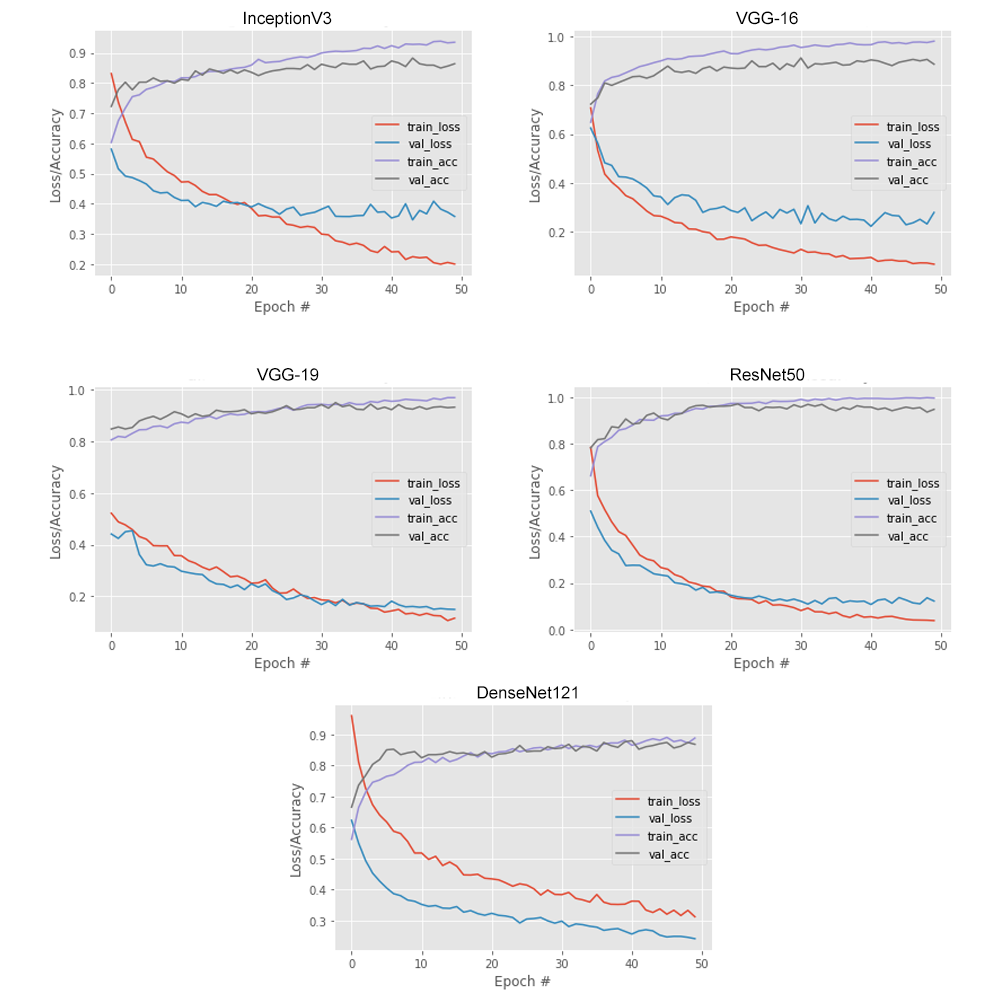
\includegraphics[scale=0.75]{images/fig-35.png}
\caption{All Model’s Train Test Accuracy and Loss Curve}
\label{fig:x All Model’s Train Test Accuracy and Loss Curve}
\end{figure}

\vspace{5mm}
\noindent Comparing All models' Accuracy and Loss graph together, we can see that VGG-19 and ResNet50 were the Good-Fit than the other models.

\vspace{5mm}
\noindent These are the Train sets, True and Predicted scores of classified and misclassified glaucoma and non-glaucoma results for each model based on the model’s train datasets prediction labels and the actual train labels. We have added a threshold of 0.5 for this train predicted visualization.

\vspace{5mm}
\noindent (the percentages are meaning the predicted train accuracy for the predicted labels calculated with the actual train labels)

\vspace{5mm}
\begin{figure}[hbt!]
\centering
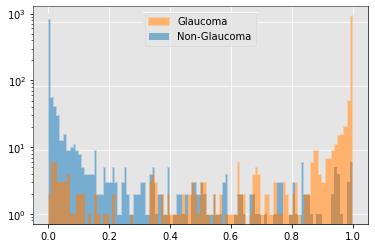
\includegraphics[scale=0.75]{images/fig-36.png}
\caption{True and Predicted Train scores of DenseNet121}
\label{fig:x True and Predicted Train scores of DenseNet121}
\end{figure}

% \centering
\begin{center}
All  151 misclassified samples (93.83\%) 

Glaucoma  74 misclassified samples (93.95\%)

Non-Glaucoma  77 misclassified samples (93.71\%)
\end{center}
\vspace{5mm}
\begin{figure}[hbt!]
\centering
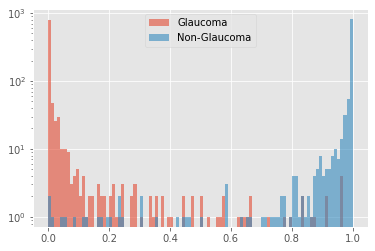
\includegraphics[scale=0.75]{images/fig-37.png}
\caption{True and Predicted Train scores of InceptionV3}
\label{fig:x True and Predicted Train scores of InceptionV3}
\end{figure}

% \centering
\begin{center}
All   48 misclassified samples (97.65\%)

Glaucoma  22 misclassified samples (97.84\%)

Non-Glaucoma  26 misclassified samples (97.45\%)
\end{center}
\vspace{5mm}
\begin{figure}[hbt!]
\centering
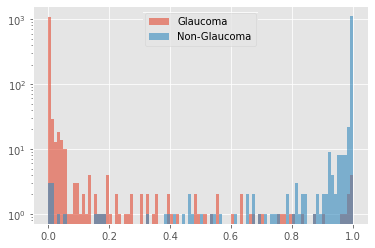
\includegraphics[scale=0.75]{images/fig-38.png}
\caption{True and Predicted Train scores of VGG-16}
\label{fig:x True and Predicted Train scores of VGG-16}
\end{figure}

\newpage
% \centering
\begin{center}
All   47 misclassified samples (98.08\%)

Glaucoma  20 misclassified samples (98.37\%)

Non-Glaucoma  27 misclassified samples (97.79\%)
\end{center}
\vspace{5mm}
\begin{figure}[hbt!]
\centering
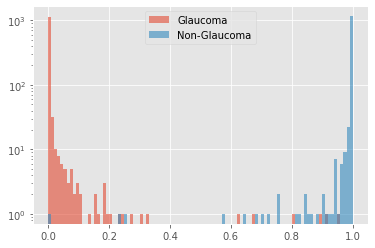
\includegraphics[scale=0.75]{images/fig-39.png}
\caption{True and Predicted Train scores of VGG-19}
\label{fig:x True and Predicted Train scores of VGG-19}
\end{figure}
\begin{center}
All   17 misclassified samples (99.31\%)

Glaucoma  14 misclassified samples (98.86\%)

Non-Glaucoma   3 misclassified samples (99.75\%)
\end{center}
\vspace{5mm}
\begin{figure}[hbt!]
\centering
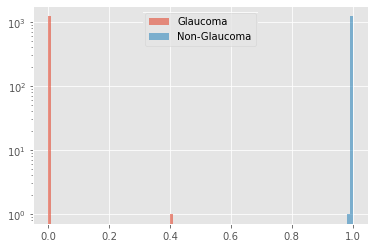
\includegraphics[scale=0.75]{images/fig-40.png}
\caption{True and Predicted Train scores of ResNet50}
\label{fig:x True and Predicted Train scores of ResNet50}
\end{figure}

\newpage
\begin{center}
All    0 misclassified samples (100.00\%)

Glaucoma   0 misclassified samples (100.00\%)

Non-Glaucoma   0 misclassified samples (100.00\%)
\end{center}
\vspace{5mm}
Now, We have called the same function that we have used for the above Train predicted labels again with the same threshold of 0.5. But for now we have used the validation datasets prediction labels. And the results were - 

\noindent \textit{(the percentages are meaning the predicted test/validation accuracy for the predicted labels calculated with the actual test/validation labels)}

\noindent \textit{( Here, G = Glaucoma and n-G = Non-Glaucoma )}

\begin{center}
\begin{table}[hbt!]
\centering
\begin{tabular}{|p{3cm}|p{3cm}|p{3cm}|c|}
\hline
% \parbox{\centering \textbf{Model}} & \parbox{\centering \textbf{All misclassified}} & \parbox{\centering \textbf{G misclassified}} & \parbox{\centering \textbf{n-G misclassified}} \\

\centering{\textbf{Model} & \centering\textbf{All misclassified} & \centering\textbf{G misclassified} & \textbf{n-G misclassified}} \\
\hline
\centering DenseNet121 & \centering 9 (86.76\%) & \centering 4 (88.24\%) & 5 (85.29\%)\\
\hline
\centering InceptionV3 & \centering 24 (85.88\%) & \centering 16 (81.18\%) & 8 (90.59\%)\\
\hline
\centering VGG-16 & \centering 8 (88.24\%) & \centering 7 (79.41\%) & 1 (97.06\%)\\
\hline
\centering VGG-19 & \centering 4 (94.12\%) & \centering 3 (91.18\%) & 1 (97.06\%)\\
\hline
\centering ResNet50 & \centering 3 (95.59\%) & \centering 1 (97.06\%) & 2 (94.12\%)\\
\hline
\end{tabular}
\caption{True and Predicted Test scores of all Model}
\label{tab:True and Predicted Test scores of all Model}
\end{table}
\end{center}



\vspace{5mm}
\noindent Now we have taken a single predicted batch from each model’s prediction with the 0.5 threshold and plotted the misclassified glaucoma and non-glaucoma images, which we will use in Lime (XAI framework) to explain later.

\noindent \textit{( Here, G = Glaucoma and n-G = Non-Glaucoma )}
\begin{center}
\begin{table}[hbt!]
\centering
\begin{tabular}{|c | c | c| c |}
\hline
\textbf{Model} & \textbf{Batch} & \textbf{G misclassified} & \textbf{n-G misclassified}}\\

\hline
DenseNet121 & 2 (32 in each) & 3 &  5\\
\hline
InceptionV3 & 2 (32 in each) & 2 & 7\\
\hline
VGG-16 & 2 (32 in each) & 2 & 3\\
\hline
VGG-19 & 2 (32 in each) & 1 & 4\\
\hline
ResNet50 & 2 (32 in each) & 0 & 3\\
\hline

\end{tabular}
\caption{True and Predicted Test scores of all Model}
\label{tab:True and Predicted Test scores of all Model}
\end{table}
\end{center}
\newpage
\vspace{5mm}
\noindent These are some of the misclassified images for all models with and undoing the existing preprocessing. Basically the model’s preprocessing for these images ruined their actual color and contrast.  Which led the model to predict wrong. By undoing the existing preprocessing we can see that for DesneNet121 the images got a little reddish and for other models, It got bluish.

\vspace{5mm}
\begin{figure}[hbt!]
\centering
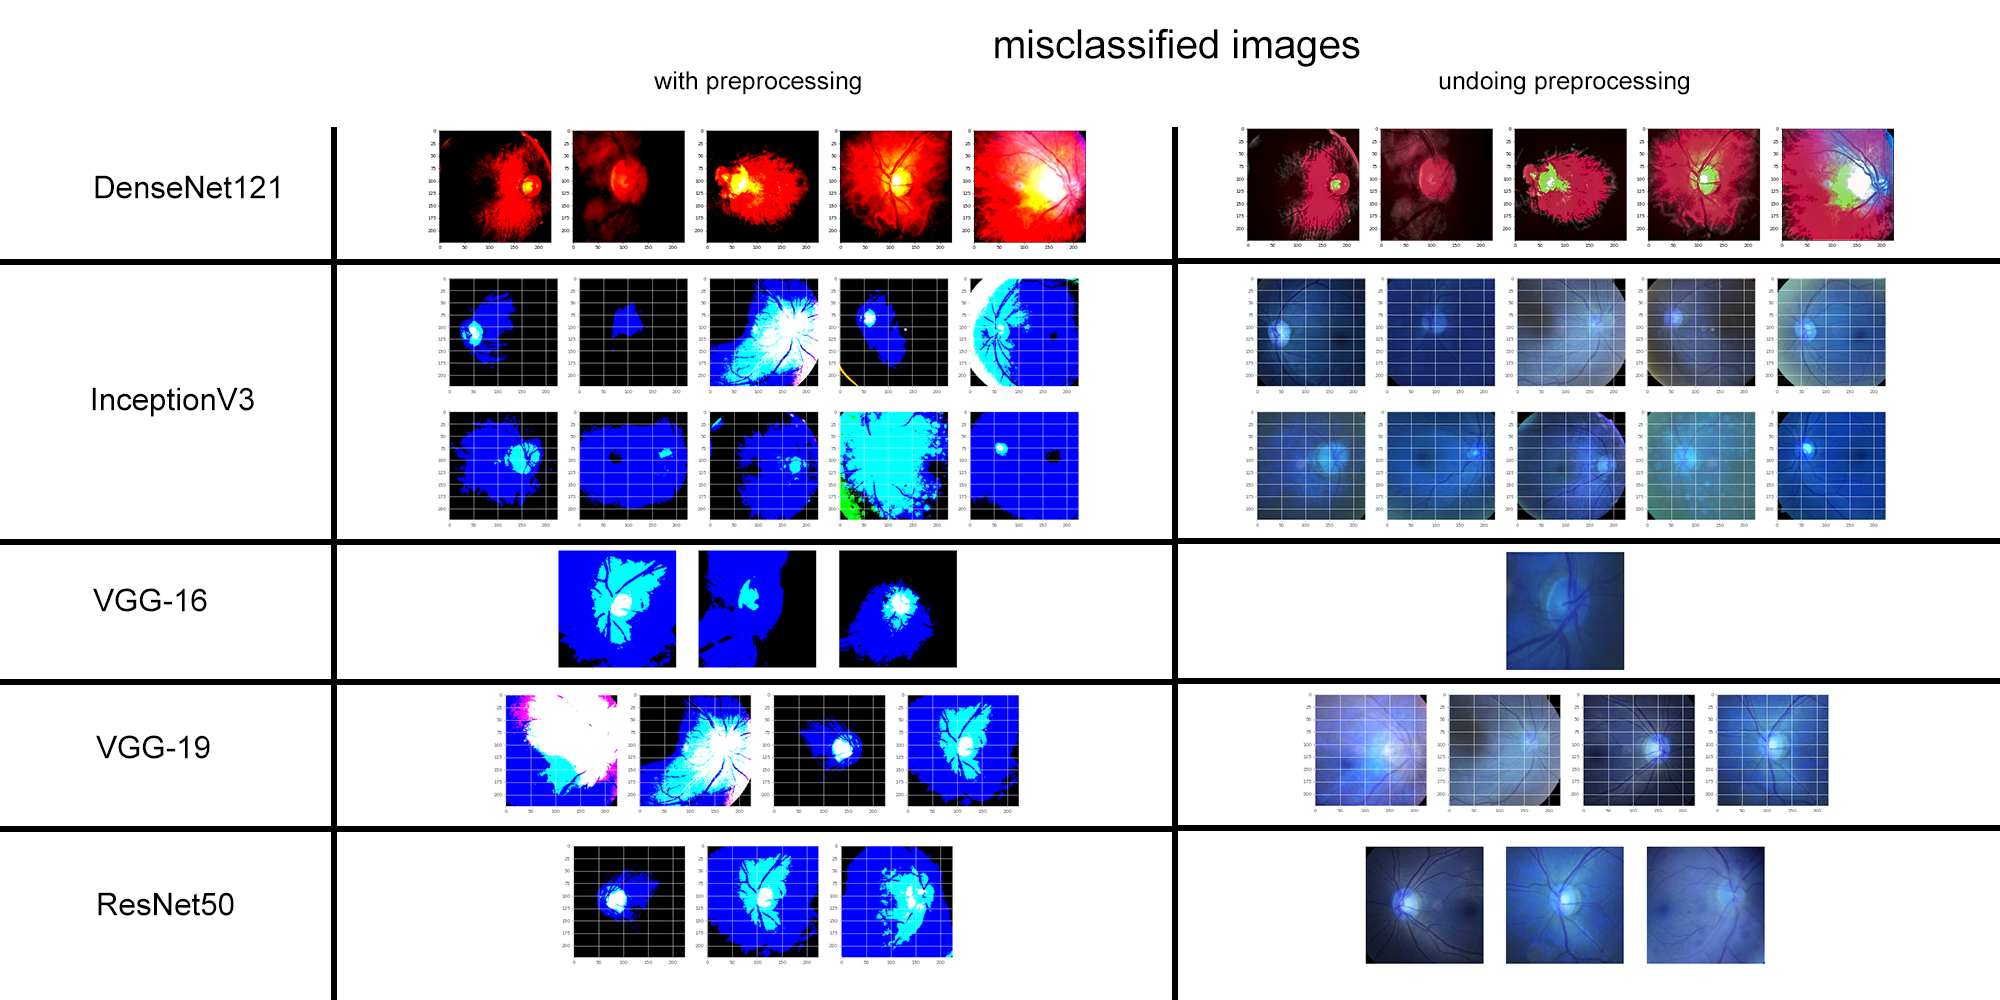
\includegraphics[scale=0.42]{images/fig-41.png}
\caption{Misclassified images for all models with and without preprocessing}
\label{fig:x True and Predicted Train scores of ResNet50}
\end{figure}

\vspace{5mm}
\noindent Now we will show the explanation for these preprocessed and misclassified images using an XAI[40] framework, \textbf{LIME}. Then we will apply Lime again on a single predicted raw fundus -image directly from the test dataset (labelled) directory to see the difference between a correctly predicted fundus image[42] and wrong predicted fundus image.
Given below are the the misclassified image with preprocessing, Superpixels focused area and the model prediction explanation by Lime in DenseNet121

\vspace{5mm}
\begin{figure}[hbt!]
\centering
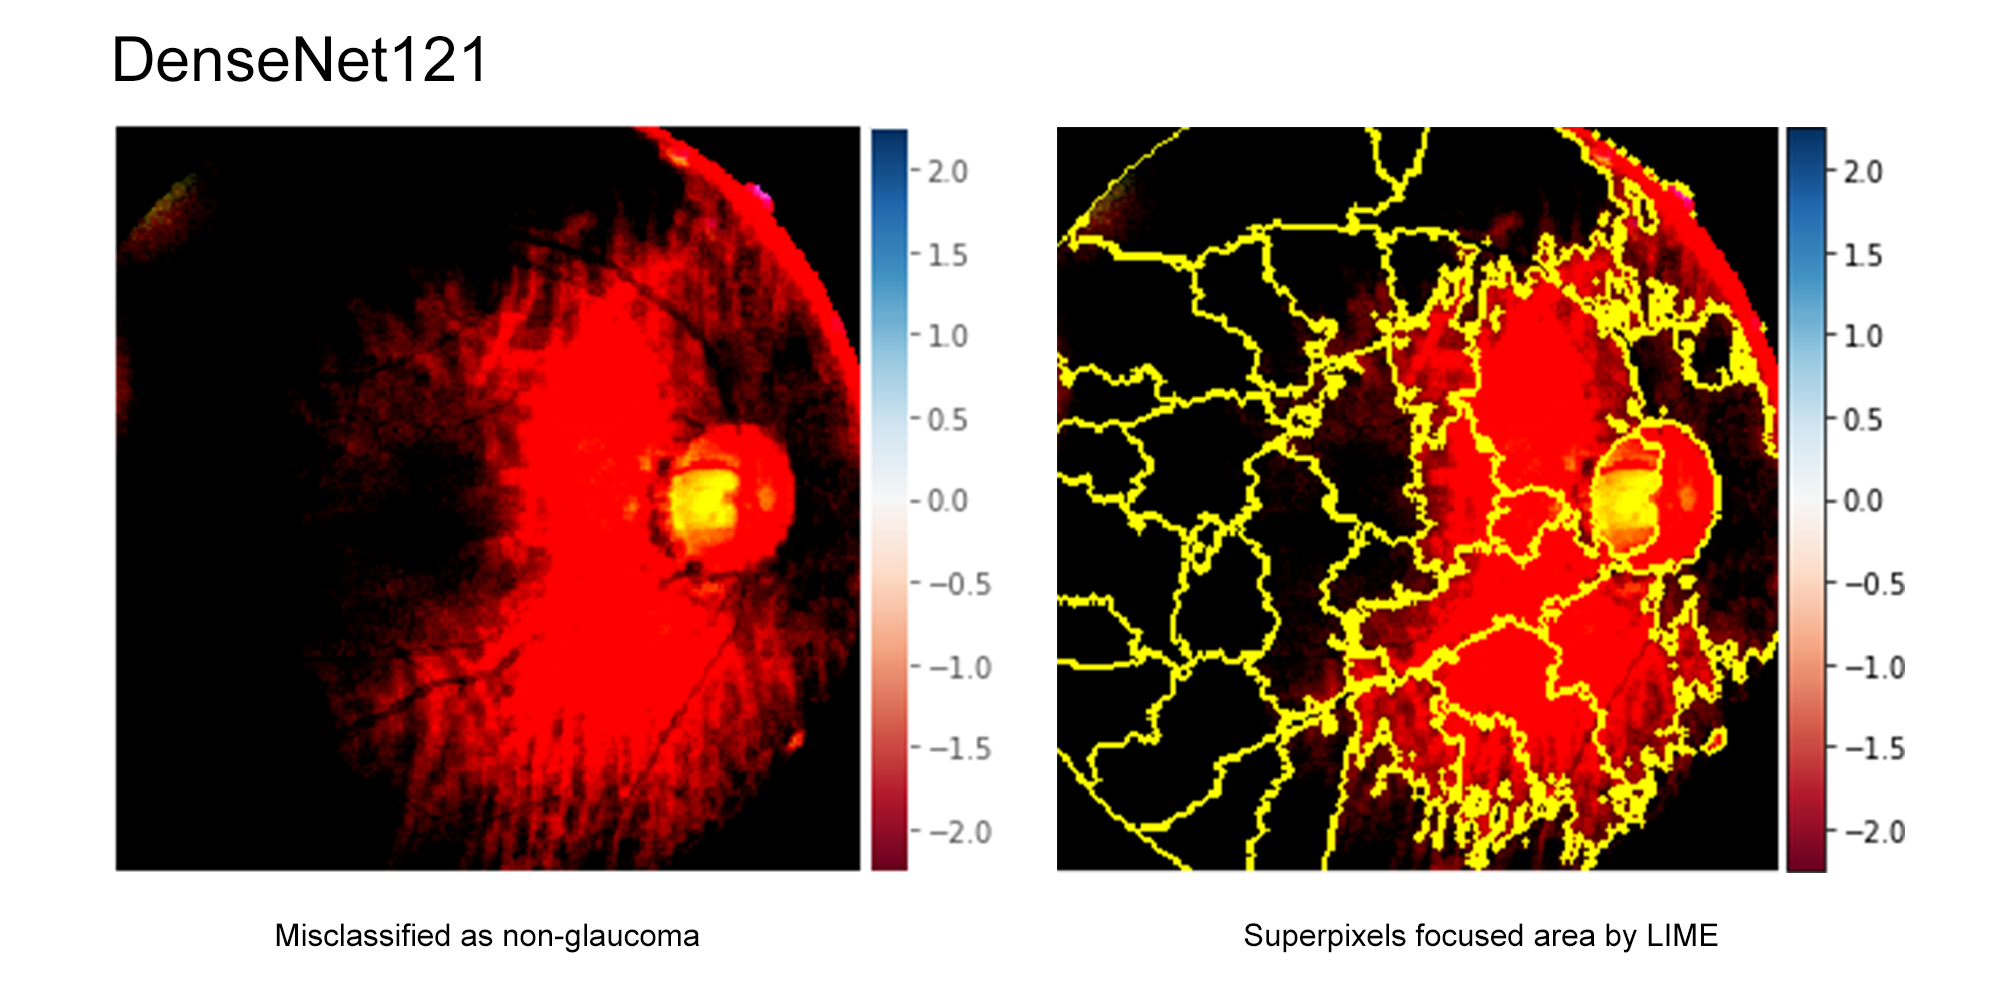
\includegraphics[scale=0.45]{images/fig-42.png}
\caption{Misclassified image with preprocessing and Superpixels focused area by Lime in DenseNet121}
\label{fig:x Misclassified image with preprocessing and Superpixels focused area by Lime in DenseNet121}
\end{figure}

\vspace{5mm}
\begin{figure}[hbt!]
\centering
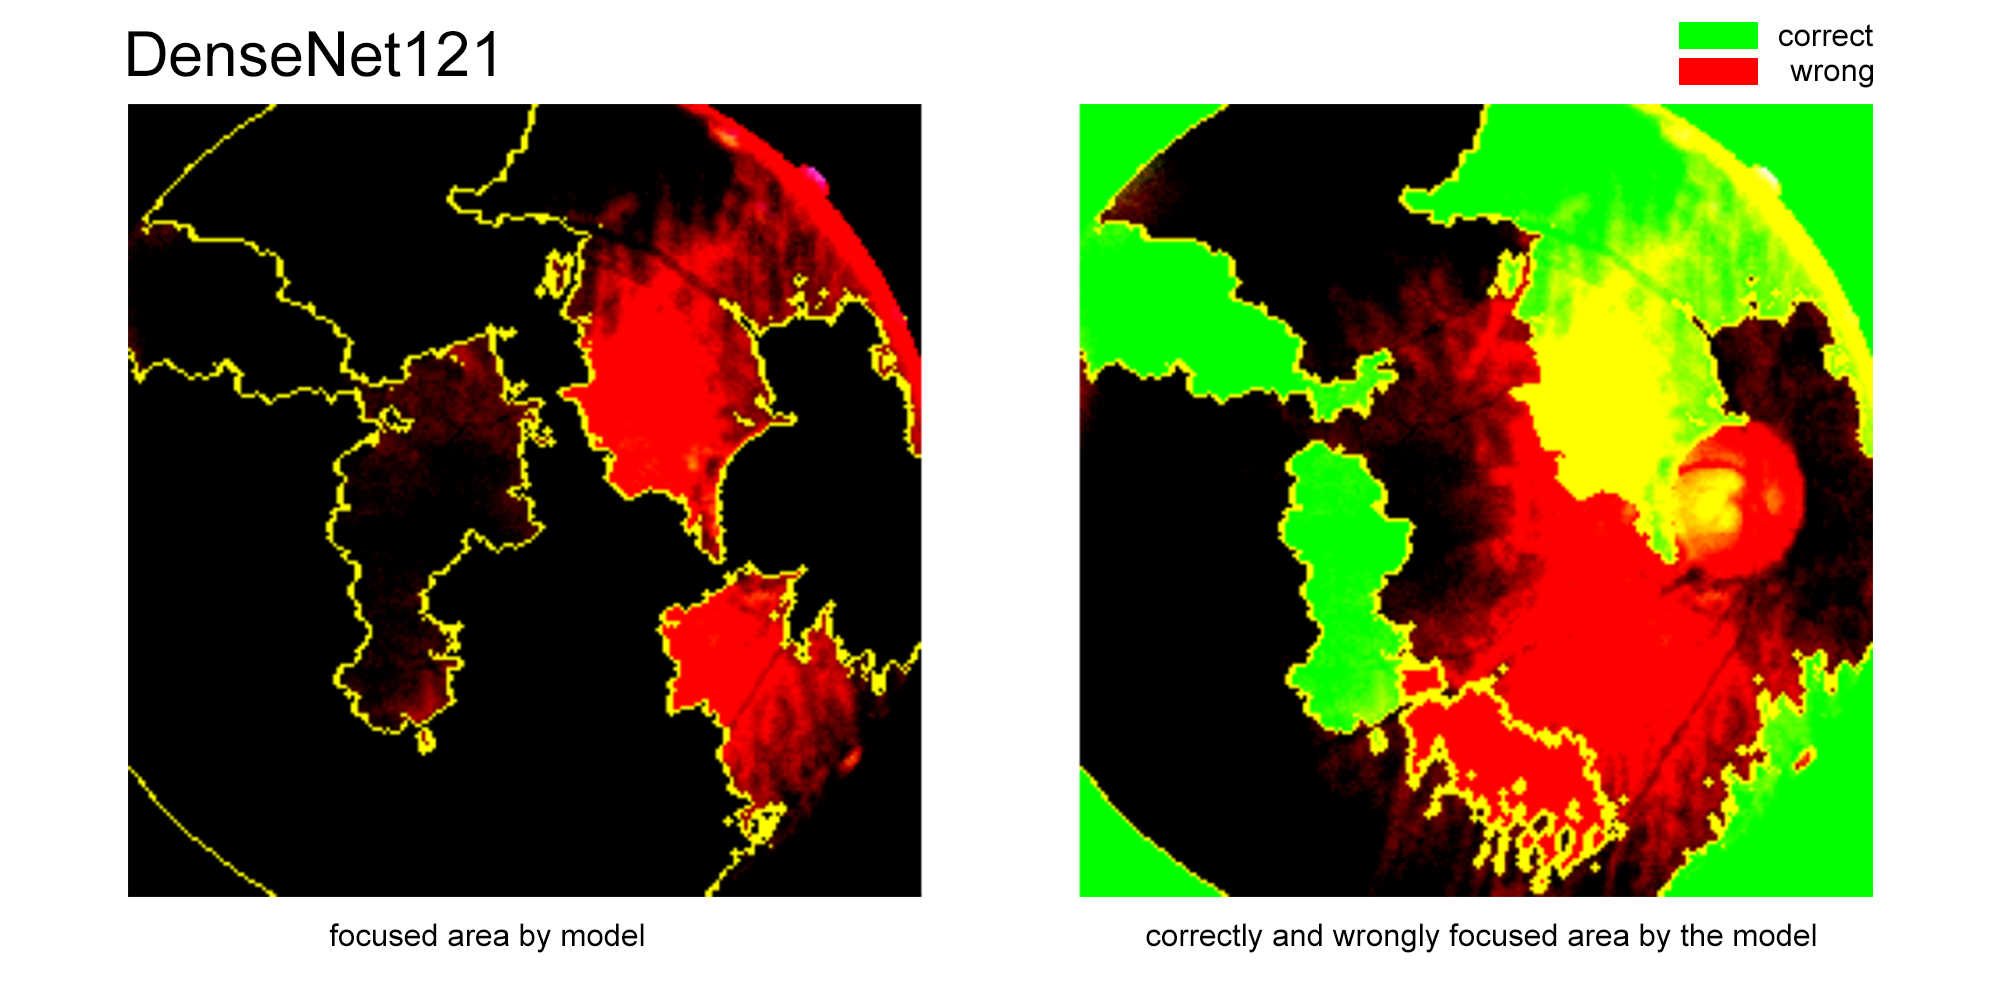
\includegraphics[scale=0.45]{images/fig-43.png}
\caption{Lime Explanation for DenseNet121}
\label{fig:x Lime Explanation for DenseNet121}
\end{figure}

\newpage
\vspace{5mm}
\noindent Given below are the the misclassified image with preprocessing, Superpixels focused area and the model prediction explanation by Lime in InceptionV3 -

\vspace{5mm}
\begin{figure}[hbt!]
\centering
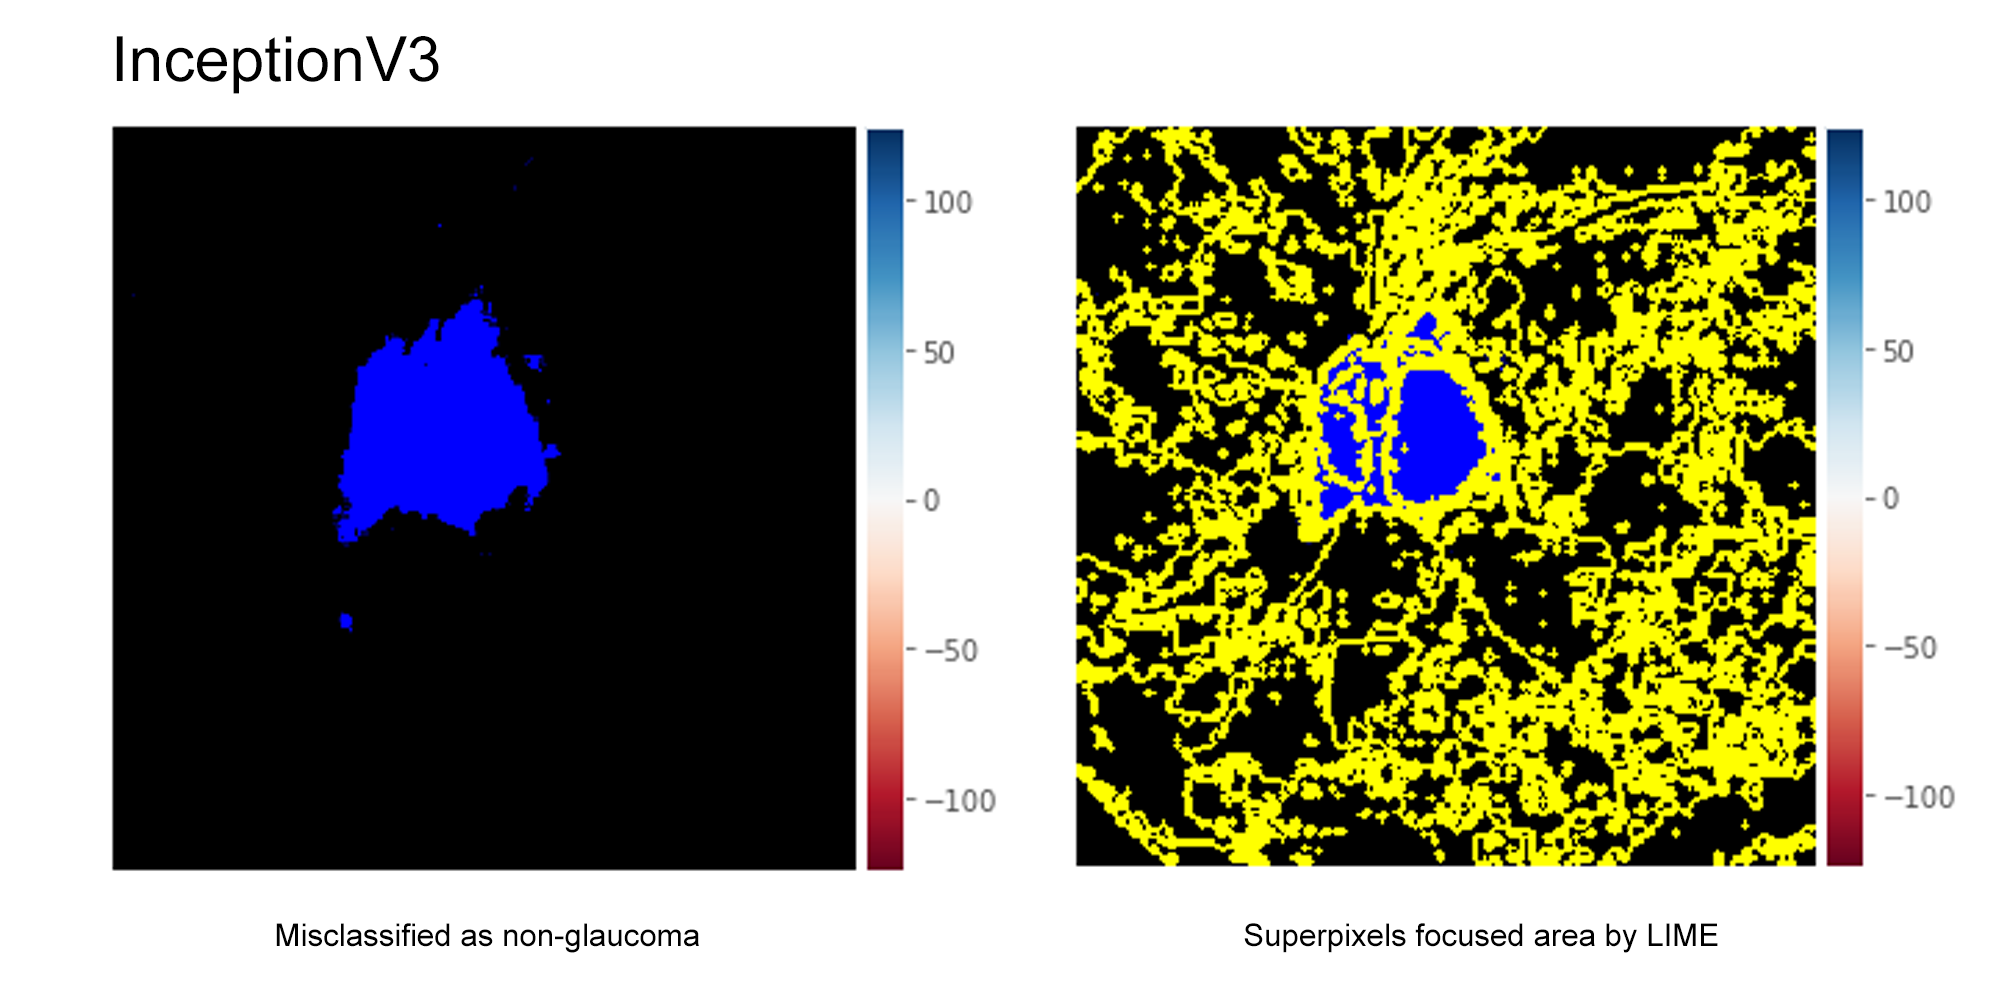
\includegraphics[scale=0.45]{images/fig-44.png}
\caption{Misclassified image with preprocessing and Superpixels focused area by Lime in InceptionV3
}
\label{fig:x Misclassified image with preprocessing and Superpixels focused area by Lime in InceptionV3
}
\end{figure}

\vspace{5mm}
\begin{figure}[hbt!]
\centering
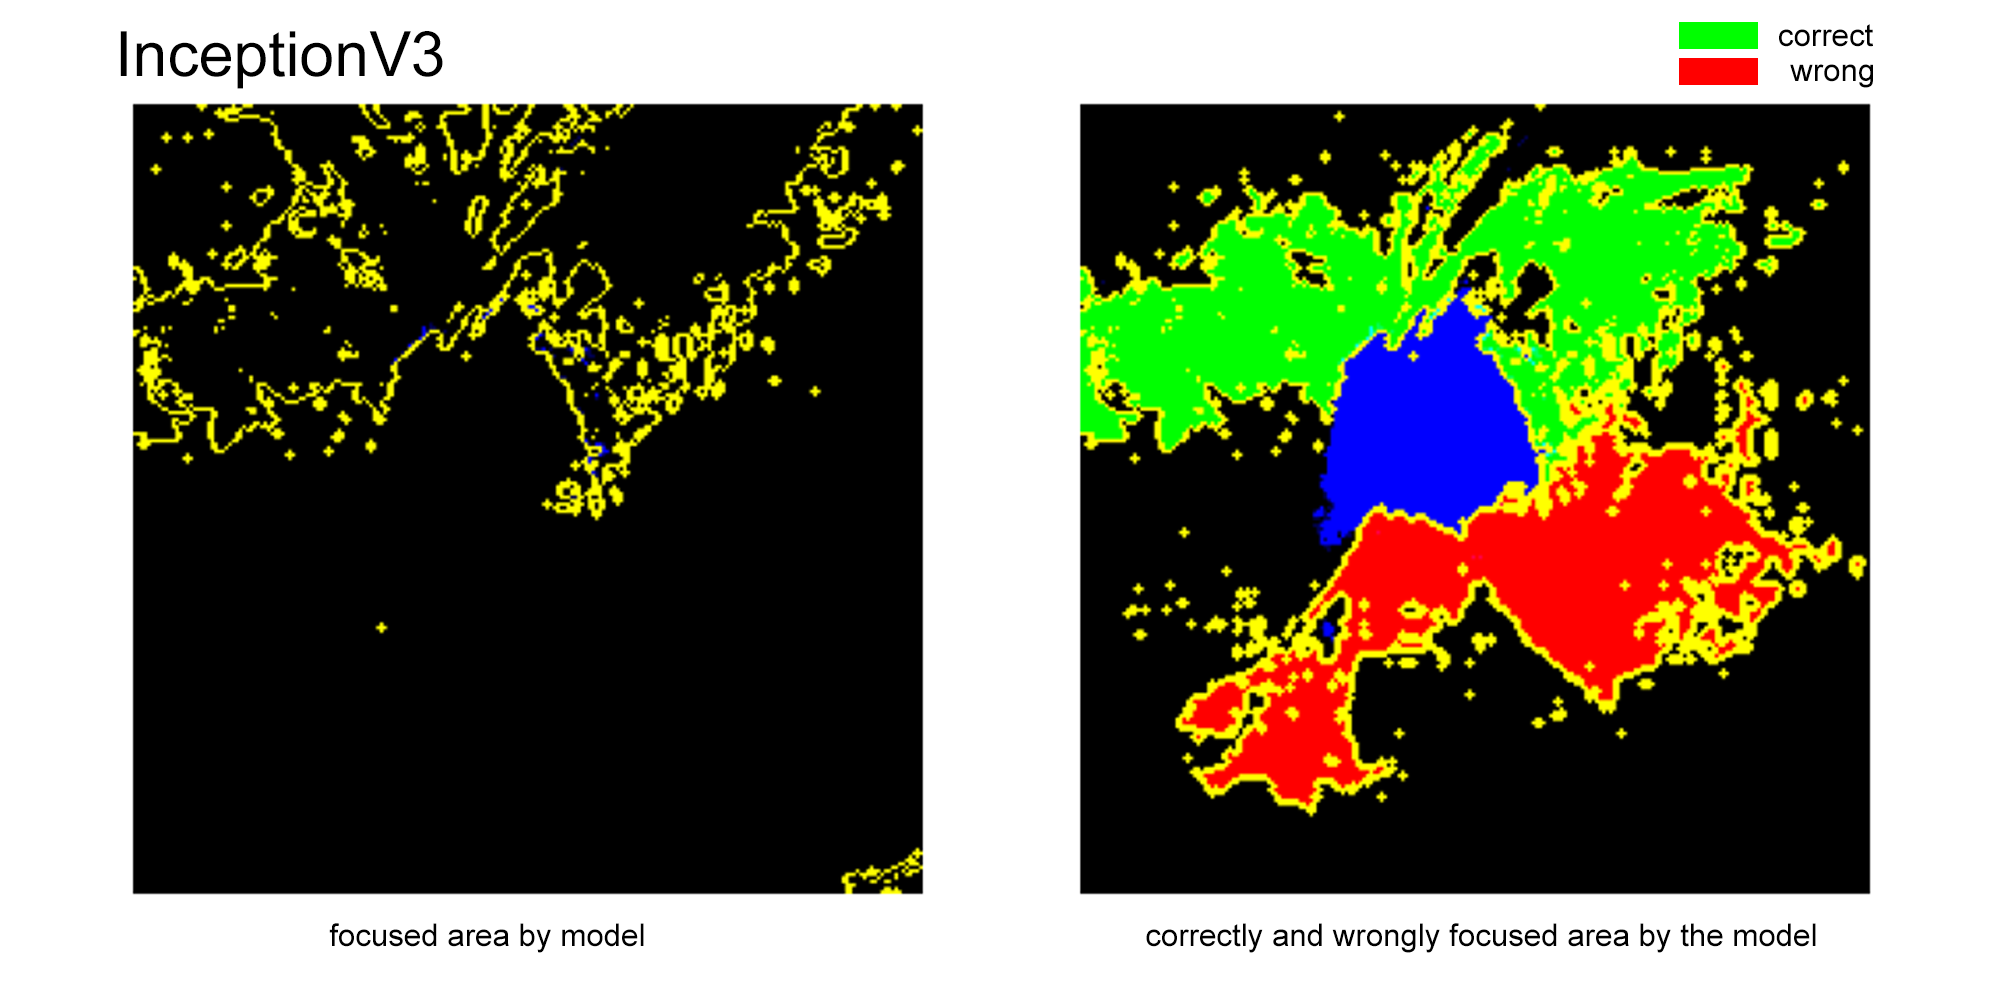
\includegraphics[scale=0.45]{images/fig-45.png}
\caption{Lime Explanation for InceptionV3}
\label{fig:x Lime Explanation for InceptionV3}
\end{figure}

\newpage
\vspace{5mm}
\noindent Given below are the the misclassified image with preprocessing, Superpixels focused area and the model prediction explanation by Lime in VGG-16 -

\vspace{5mm}
\begin{figure}[hbt!]
\centering
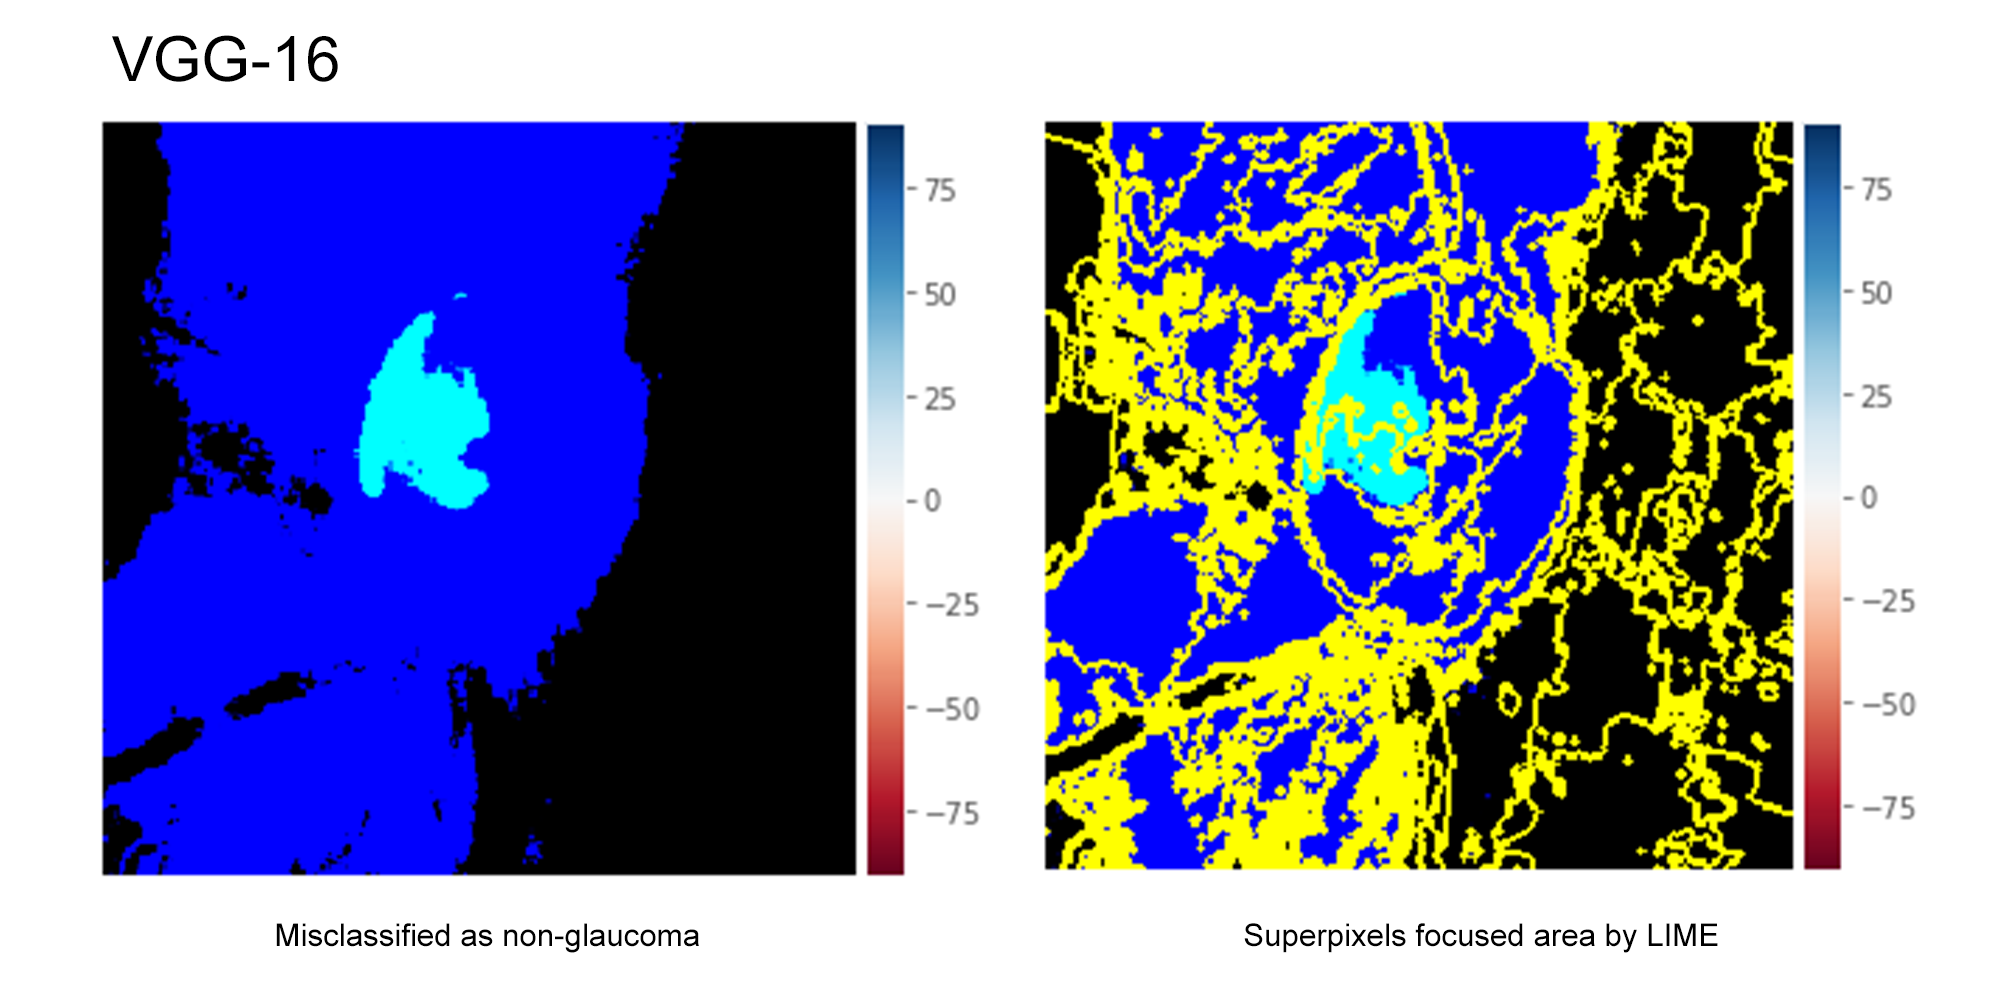
\includegraphics[scale=0.45]{images/fig-46.png}
\caption{Misclassified image with preprocessing and Superpixels focused area by Lime in VGG-16}
\label{fig:x Misclassified image with preprocessing and Superpixels focused area by Lime in VGG-16}
\end{figure}

\vspace{5mm}
\begin{figure}[hbt!]
\centering
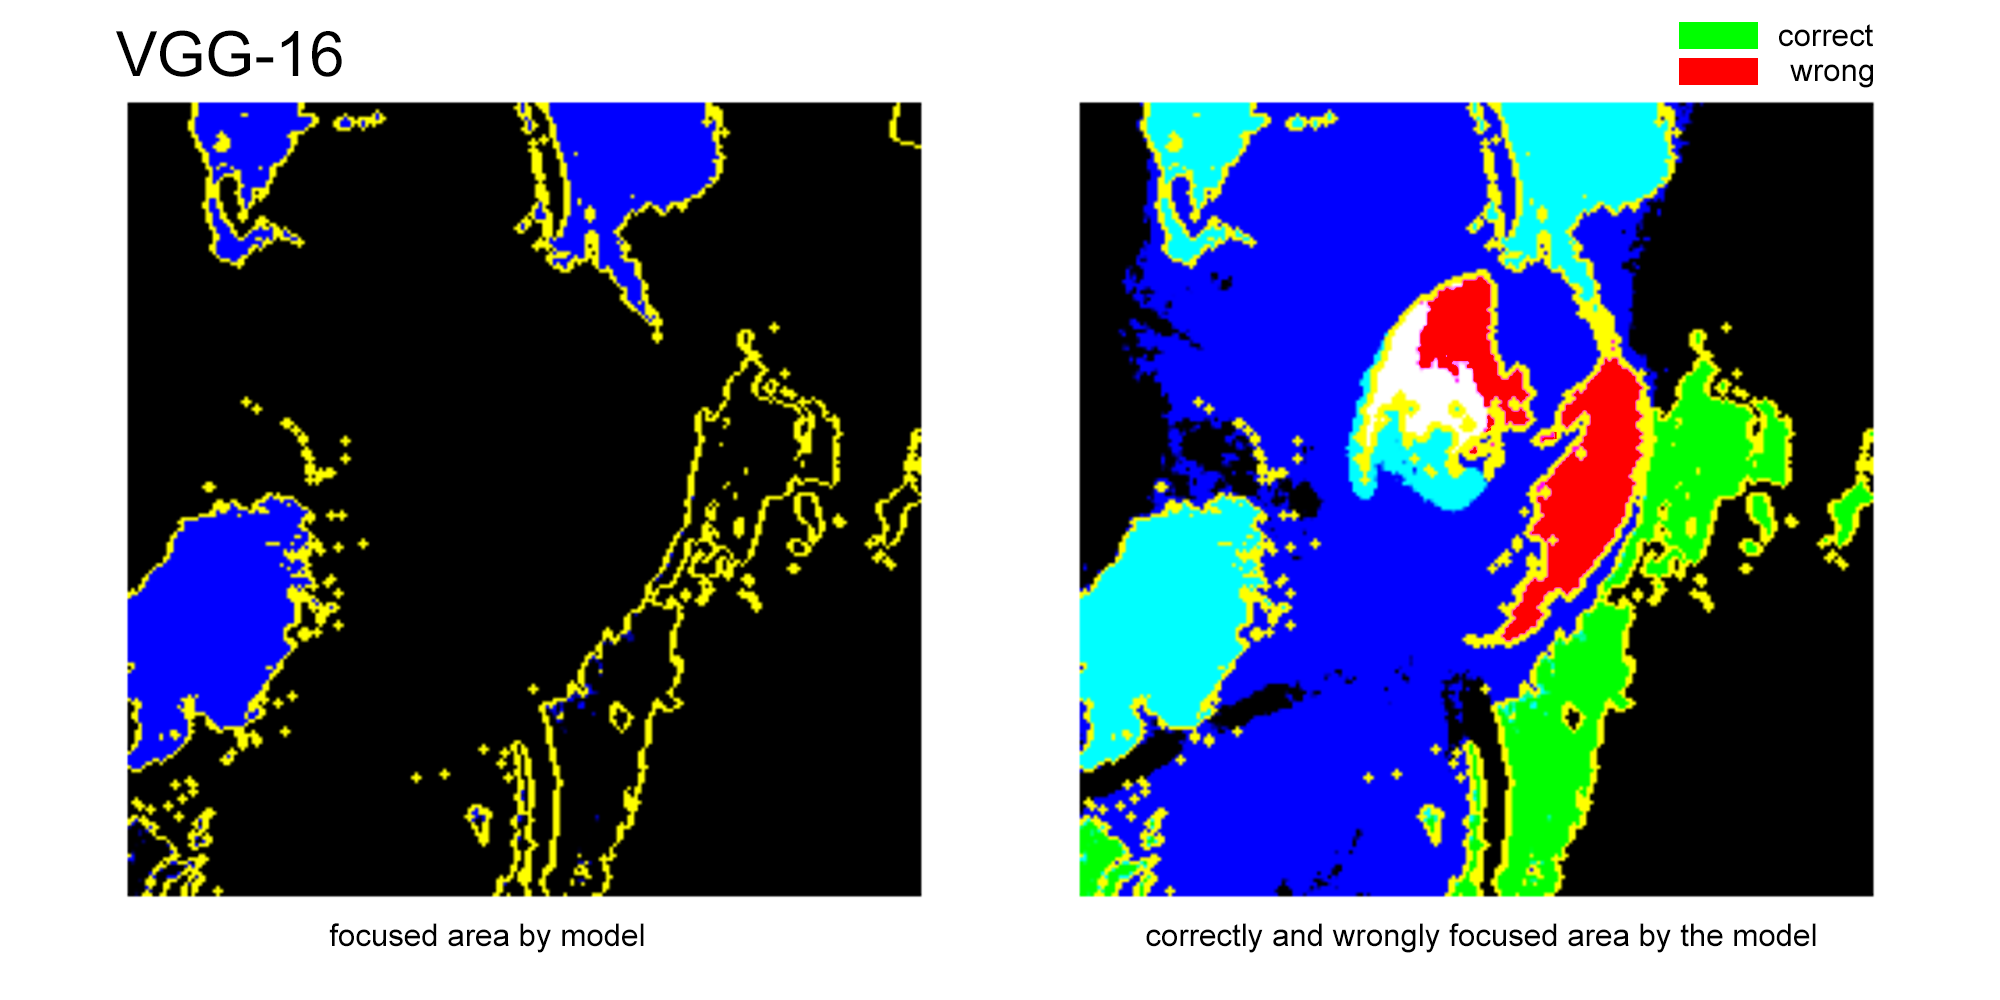
\includegraphics[scale=0.45]{images/fig-47.png}
\caption{Lime Explanation for VGG-16}
\label{fig:x Lime Explanation for VGG-16}
\end{figure}

\newpage
\vspace{5mm}
\noindent Given below are the the misclassified image with preprocessing, Superpixels focused area and the model prediction explanation by Lime in VGG-19 -

\vspace{5mm}
\begin{figure}[hbt!]
\centering
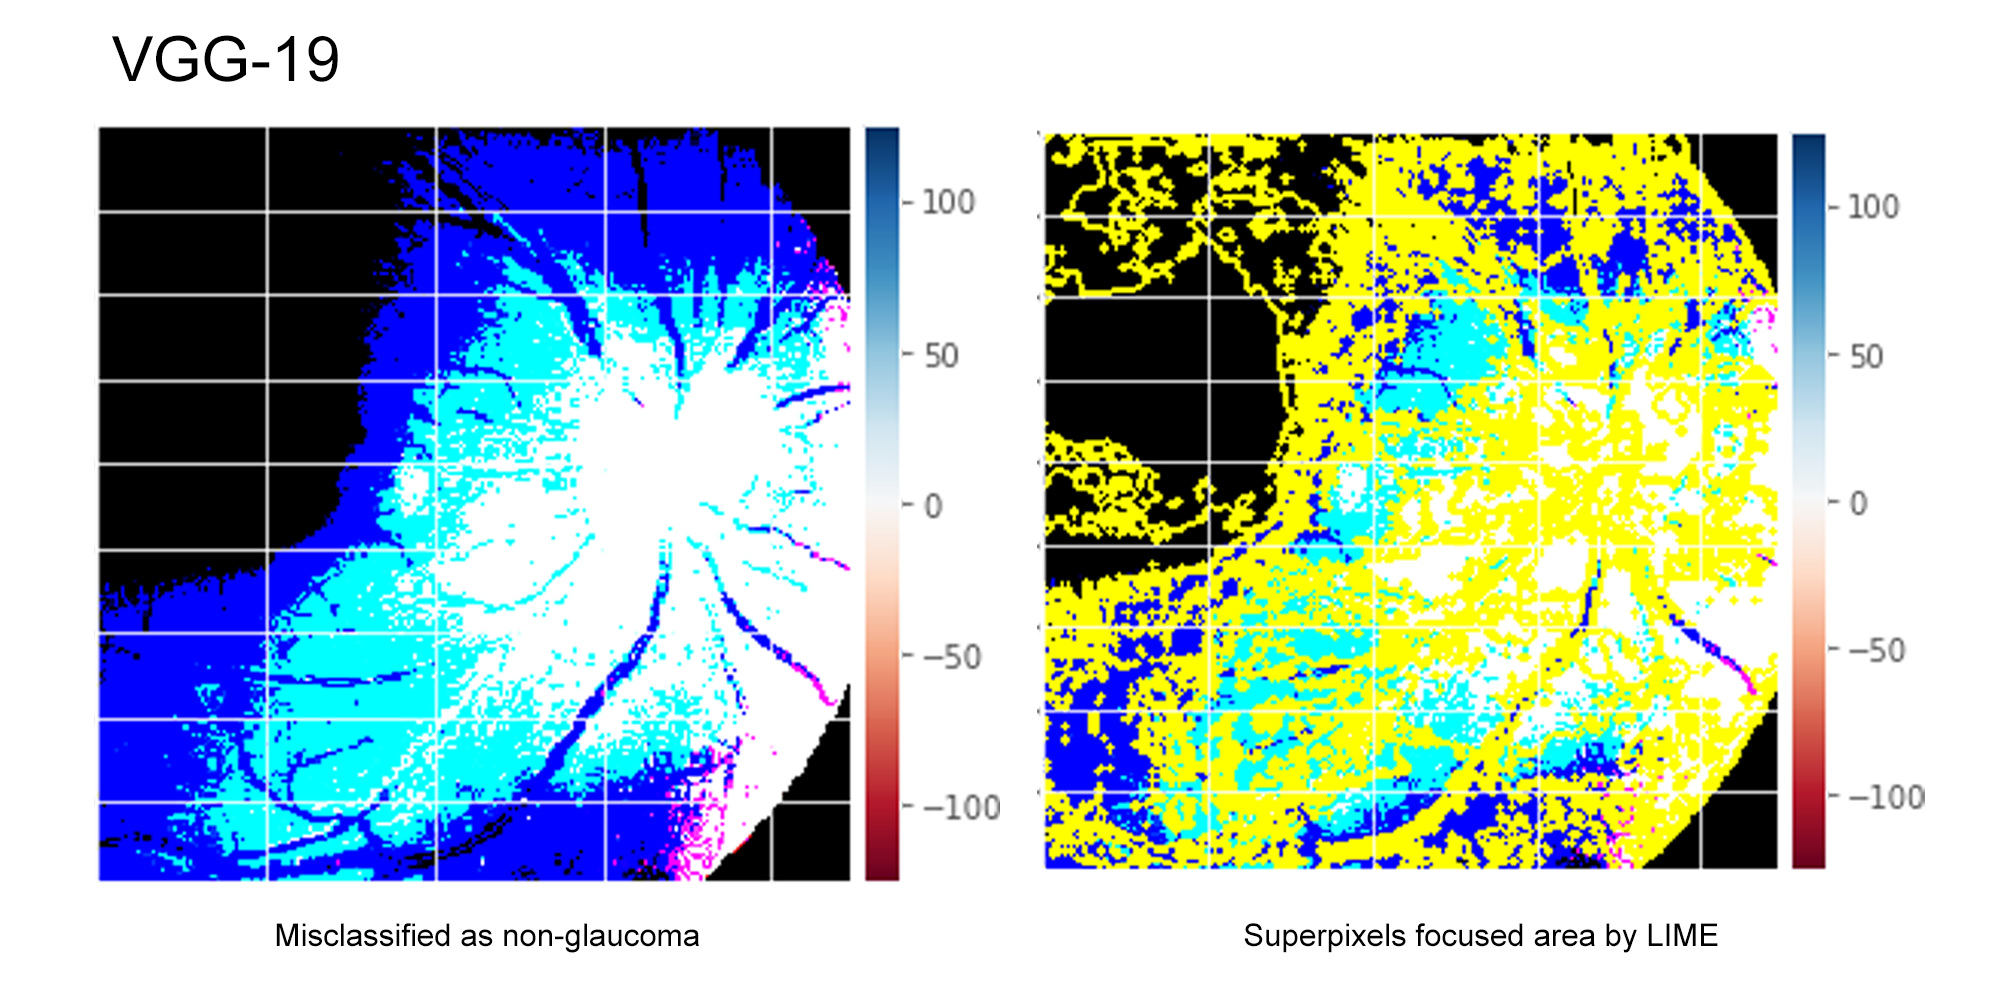
\includegraphics[scale=0.45]{images/fig-48.png}
\caption{Misclassified image with preprocessing and Superpixels focused area by Lime in VGG-19}
\label{fig:x Misclassified image with preprocessing and Superpixels focused area by Lime in VGG-19}
\end{figure}

\vspace{5mm}
\begin{figure}[hbt!]
\centering
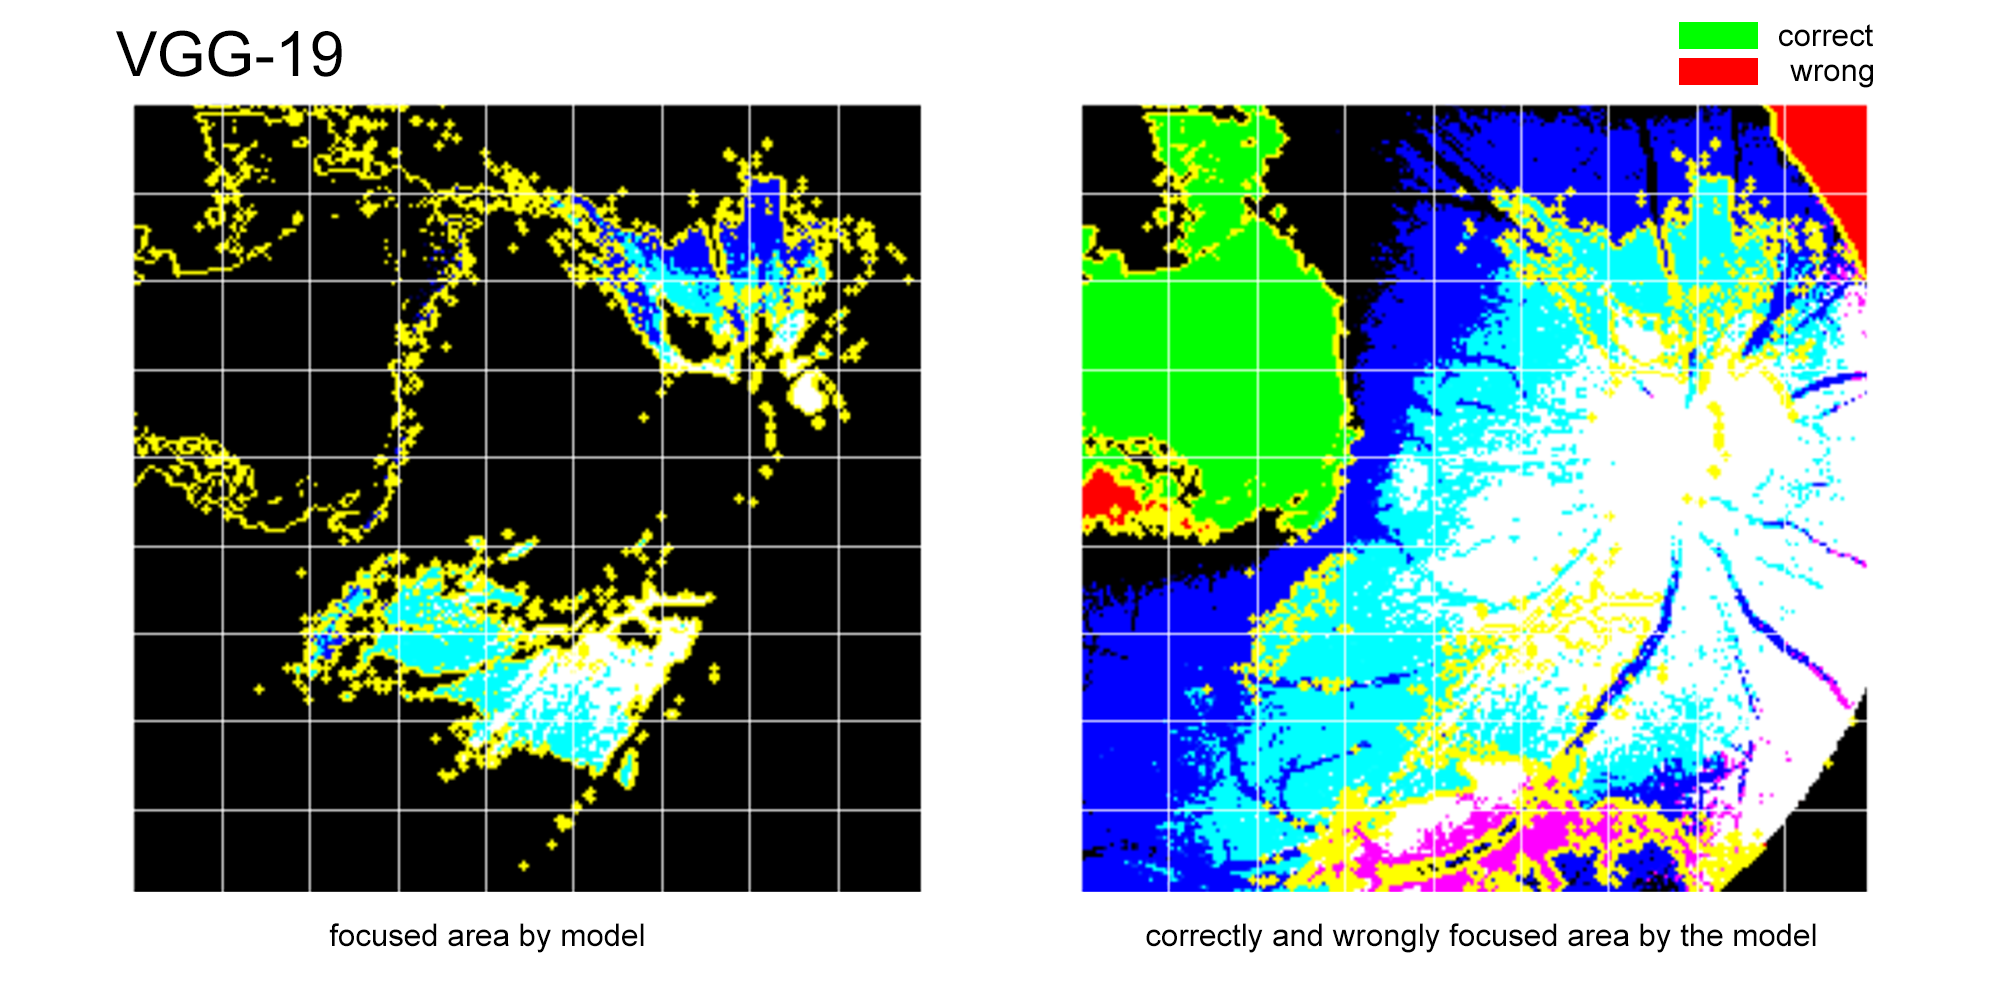
\includegraphics[scale=0.45]{images/fig-49.png}
\caption{Lime Explanation for VGG-19}
\label{fig:x Lime Explanation for VGG-19}
\end{figure}

\newpage
\vspace{5mm}
\noindent Given below are the the misclassified image with preprocessing, Superpixels focused area and the model prediction explanation by Lime in ResNet50 -

\vspace{5mm}
\begin{figure}[hbt!]
\centering
\includegraphics[scale=0.45]{images/fig-50.png}
\caption{Misclassified image with preprocessing and Superpixels focused area by Lime in ResNet50}
\label{fig:x Misclassified image with preprocessing and Superpixels focused area by Lime in ResNet50}
\end{figure}

\vspace{5mm}
\begin{figure}[hbt!]
\centering
\includegraphics[scale=0.45]{images/fig-51.png}
\caption{Lime Explanation for ResNet50}
\label{fig:x Lime Explanation for ResNet50}
\end{figure}

\newpage
\vspace{5mm}
Now for the single predicted raw fundus image -

\vspace{5mm}
\begin{figure}[hbt!]
\centering
\includegraphics[scale=0.20]{images/fig-52.png}
\caption{Lime Explanation for all models single image predictions}
\label{fig:x Lime Explanation for all models single image predictions}
\end{figure}

\newpage
\section{Result}
These are the single image predictions of all models - 

\noindent\textit{( here outputs are given in [n,m] format, where “m” means glaucoma score and “n” means non-glaucoma score )}

\vspace{5mm}
\begin{figure}[hbt!]
\centering
\includegraphics[scale=0.6]{images/fig-53.png}
\caption{Single Image Predictions for all Model}
\label{fig:x Single Image Predictions for all Model}
\end{figure}

\newpage
\vspace{5mm}
\noindent\textit{These are batch (50 images/batch) image predictions of all models - ( here [1,0] means glaucoma and [0,1] means non-glaucoma )}


\vspace{5mm}
\begin{figure}[hbt!]
\centering
\includegraphics[scale=0.6]{images/fig-54.png}
\caption{Batch Predictions for DenseNet121}
\label{fig:x Batch Predictions for DenseNet121}
\end{figure}

\vspace{5mm}
\begin{figure}[hbt!]
\centering
\includegraphics[scale=0.6]{images/fig-55.png}
\caption{Batch Predictions for InceptionV3}
\label{fig:x Batch Predictions for InceptionV3}
\end{figure}

\newpage
\vspace{5mm}
\noindent\textit{These are batch (50 images/batch) image predictions of all models - ( here [1,0] means glaucoma and [0,1] means non-glaucoma )}

\vspace{5mm}
\begin{figure}[hbt!]
\centering
\includegraphics[scale=0.6]{images/fig-56.png}
\caption{Batch Predictions for VGG-16}
\label{fig:x Batch Predictions for VGG-16}
\end{figure}

\vspace{5mm}
\begin{figure}[hbt!]
\centering
\includegraphics[scale=0.6]{images/fig-57.png}
\caption{Batch Predictions for VGG-19}
\label{fig:x Batch Predictions for VGG-19}
\end{figure}

\vspace{5mm}
\begin{figure}[hbt!]
\centering
\includegraphics[scale=0.6]{images/fig-58.png}
\caption{ Batch Predictions for ResNet50}
\label{fig:x  Batch Predictions for ResNet50}
\end{figure}



\nomenclature{$OOP$}{Object Oriented Programming}
\nomenclature{$AdaM$}{Adaptive Momentum}


\chapter{Conclusion}
%\section{Conclusion}
\section{Conclusion} 
In this research, to attain the ultimate objective of our study in Glaucoma Diagnosis, the Black
Box model was defined using Explainable Artificial Intelligence (XAI). As we have introduced
our work we have done so far in this research paper. Through this research, we were led to more
glaucoma diagnosis acceptability. Notably, glaucoma can take away the vision of a patient which
is why it’s more important to work for a better solution for early stage detection of glaucoma
disease. For this reason, using the XAI, recognition, and treatment of Glaucoma can bring an
immense change in the system which is very important, as reducing the number of blindness
caused by glaucoma through early proper detection and treatment of the disease is going to be a
huge success to celebrate. Because around the world 1 out of 15 people are blind because of it.
Statistics show that even with the treatment 15\% to 20\% of the patients become blind. To serve
our purpose we have used VGG-16, VGG-19, DenseNet121, InceptionV3 and ResNet50 models
for our study. Every model was compiled with Adam optimizer with the learning rate of 1e-5 in
50 epochs. If we look at the score which is validation accuracy for our models we can see that in
InceptionV3 we got 86.4\% accuracy, in DenseNet121 we got 86.8\% accuracy, in ResNet50 we
got 94.7\% accuracy, in VGG-19 we got 93.3\% accuracy and lastly in VGG-16 we got 88.6\%
accuracy. As the results showed, after 50 epochs, RestNet50 got the highest score among the
other models with a validation accuracy of 94.7\%. Afterwards we compared all models' accuracy
and loss graph together, where we can see that VGG-19 and ResNet50 were the Good-Fit than
the other models. So for our purpose we are proposing to use the LIME for getting rid of the very
lessened percentage in accuracy. Thereupon, in this research authors mentioned and showed how
they have used Deep Neural Network Leveraging Explainable Artificial Intelligence to reduce
the amount of Glaucoma Patients through early detection. Since there still is no known approach
to prevent glaucoma, glaucoma-related blindness or major visual loss can be avoided if the
condition is detected at an early stage. As now the AI has been improved and gained reliability in
the medical sector so as per research it can be prevented by early detection. To sum up, we can
say this research has achieved the goal to bring more accuracy, reliability and committed to
improving more in Glaucoma diagnosis to make a difference in human life and contribute
accordingly.

%\section{Bibliography}
\justifying
\section*{Bibliography} 
\noindent[1] Salam, A. A., Khalil, T., Akram, M. U., Jameel, A., & Basit, I. (2016). Automated detection of glaucoma using structural and non structural features. SpringerPlus, 5(1).\\ https://doi.org/10.1186/s40064-016-3175-4

\vspace{5mm}
\noindent[2] Ran, A., & Cheung, C. Y. (2021). Deep Learning-Based Optical Coherence Tomography and Optical Coherence Tomography Angiography Image Analysis: An Updated Summary. Asia-Pacific Journal of Ophthalmology, 10(3), 253–260. 

\noindent https://doi.org/10.1097/apo.0000000000000405

\vspace{5mm}
\noindent[3] Aleci, C. (2020). Detection of Visual Field Loss Progression in Glaucoma: An Overview and Food for Thought. Ophthalmology Research: An International Journal, 16–24.\\
https://doi.org/10.9734/or/2020/v13i130158

\vspace{5mm}
\noindent[4] Saha, S., Wang, Z., Sadda, S., Kanagasingam, Y., & Hu, Z. (2020). Visualizing and understanding inherent features in SD‐OCT for the progression of age‐related macular degeneration using deconvolutional neural networks. Applied AI Letters, 1(1). 

\noindent https://doi.org/10.1002/ail2.16
 
\vspace{5mm}
\noindent[5] Civit-Masot, J., Dominguez-Morales, M. J., Vicente-Diaz, S., & Civit, A. (2020). Dual Machine-Learning System to Aid Glaucoma Diagnosis Using Disc and Cup Feature Extraction. IEEE Access, 8, 127519–127529. 

\noindent https://doi.org/10.1109/access.2020.3008539

\vspace{5mm}
\noindent[6] Diabetic Retinopathy | National Eye Institute. (2021, July 30). National Eye Institute. 

\noindent https://www.nei.nih.gov/learn-about-eye-health/eye-conditions-and-diseases/diabetic-retinopathy

\vspace{5mm}
\noindent[7] Types of Glaucoma.(2020, June 2). Glaucoma Research Foundation. 

\noindent https://www.glaucoma.org/glaucoma/types-of-glaucoma.php#:\%7E:text=There\%20are\% 20several\%20types\%20of,or\%20pressure\%20inside\%20the\%20eye

\vspace{5mm}
\noindent[8] Saba, T., Khan, M. W., Yasmin, M., & Sharif, M. (2017). CDR based glaucoma detection using fundus images: a review. International Journal of Applied Pattern Recognition, 4(3), 261. 

\noindent https://doi.org/10.1504/ijapr.2017.10007613

\vspace{5mm}
\noindent[9] Thakoor, K. A., Li, X., Tsamis, E., Sajda, P., & Hood, D. C. (2019). Enhancing the Accuracy of Glaucoma Detection from OCT Probability Maps using Convolutional Neural Networks. 2019 41st Annual International Conference of the IEEE Engineering in Medicine and Biology Society (EMBC). 

\noindent https://doi.org/10.1109/embc.2019.8856899

\vspace{5mm}
\noindent[10]  Lim, T. C., Chattopadhyay, S., & Acharya, U. R. (2012). A survey and comparative study on the instruments for glaucoma detection. Medical Engineering & Physics, 34(2), 129–139. 

\noindent https://doi.org/10.1016/j.medengphy.2011.07.030

\vspace{5mm}
\noindent[11] Muddamsetty, S. M., Jahromi, M. N. S., & Moeslund, T. B. (2021b). Expert Level Evaluations for Explainable AI (XAI) Methods in the Medical Domain. Pattern Recognition. ICPR International Workshops and Challenges, 35–46. 

\noindent https://doi.org/10.1007/978-3-030-68796-0_3

\vspace{5mm}
\noindent[12] Abbas, Q. (2017). Glaucoma-Deep: Detection of Glaucoma Eye Disease on Retinal Fundus Images using Deep Learning. International Journal of Advanced Computer Science and Applications, 8(6). 

\noindent https://doi.org/10.14569/ijacsa.2017.080606

\vspace{5mm}
\noindent[13]  Dervisevic, E., Pavljasevic, S., Dervisevic, A., & Kasumovic, A. (2016). Challenges In Early Glaucoma Detection. Medical Archives, 70(3), 203. 

\noindent https://doi.org/10.5455/medarh.2016.70.203-207

\vspace{5mm}
\noindent[14]  R. Asaoka, H. Murata, A. Iwase, M. Araie, “Detecting preperimetric Glaucoma with Standard Automated Perimetry Using a Deep Learning Classifier,” Ophthalmology, vol. 123, pp. 1974–1980, September 2016.

\vspace{5mm}
\noindent[15]  Mayro, E.L., Wang, M., Elze, T. et al. The impact of artificial intelligence in the diagnosis and management of glaucoma. Eye 34, 1–11 (2020). 

\noindent https://doi.org/10.1016/j.ophtha.2016.05.029

\vspace{5mm}
\noindent[16]  Shabbir, A., Rasheed, A., Shehraz, H., Saleem, A., Zafar, B., Sajid, M., Ali, N., Dar, S. H., & Shehryar, T. (2021). Detection of glaucoma using retinal fundus images: A comprehensive review. Mathematical Biosciences and Engineering, 18(3), 2033–2076. 

\noindent https://doi.org/10.3934/mbe.2021106

\vspace{5mm}
\noindent[17] Brown, J. M., & Leontidis, G. (2021). Deep learning for computer-aided diagnosis in ophthalmology: a review. State of the Art in Neural Networks and their Applications, 219-237.


\noindent https://www.sciencedirect.com/science/article/pii/B9780128197400000115

\vspace{5mm}
\noindent[18] Sau, P. C., Gupta, M., & Kumar, D. (2021). A Comparative Study: Glaucoma Detection Using Deep Neural Networks. In Proceedings of International Conference on Big Data, Machine Learning and their Applications (pp. 85-97). Springer, Singapore.

\noindent https://link.springer.com/chapter/10.1007/978-981-15-8377-3_8

\vspace{5mm}
\noindent[19] Greco, A., Rizzo, M. I., De Virgilio, A., Gallo, A., Fusconi, M., de Vincentiis, M. (2016). Emerging concepts in Glaucoma and review of the literature. The American Journal of Medicine (2016).

\noindent https://doi.org/10.1016/j.amjmed.2016.03.038

\vspace{5mm}
\noindent[20] Pascolini, D., & Mariotti, S. P. (2012). Global estimates of visual impairment: 2010. British Journal of Ophthalmology, 96(5), 614-618.

\noindent https://bjo.bmj.com/content/96/5/614.short

\vspace{5mm}
\noindent[21] Goldbaum MH, Sample PA, White H, Colt B, Raphaelian P, Fechtner RD, et al. Interpretation of automated perimetry for glaucoma by neural network. Invest Ophthalmol Vis Sci. 1994;35:3362–73. 


\noindent\url{https://www.researchgate.net/publication/15141759_Interpretation_of_automated\\_perimetry_for_glaucoma_by_neural_network}

\vspace{5mm}
\noindent[22]  Murphy, A. M., & Moore, C. M. M. (2020). Fully connected neural network. 

\noindent https://radiopaedia.org/articles/fully-connected-neural-network

\vspace{5mm}
\noindent[23] Brownlee, J. (2020, August 14). What is Deep Learning? Machine Learning Mastery. 

\noindent https://machinelearningmastery.com/what-is-deep-learning/

\vspace{5mm}
\noindent[24] Khan, S. M. K. (2021, January 3). Papers with Code - LAG Dataset. The Lancet. 

\noindent https://paperswithcode.com/dataset/lag

\vspace{5mm}
\noindent[25] How to fine-tune your artificial intelligence algorithms 

\noindent https://www.allerin.com/blog/how-to-fine-tune-your-artificial-intelligence-algorithms

\vspace{5mm}
\noindent[26] Saxena, A., Vyas, A., Parashar, L., & Singh, U. (2020, July). A glaucoma detection using a convolutional neural network. In 2020 International Conference on Electronics and Sustainable Communication Systems (ICESC) (pp. 815-820). IEEE.

\noindent https://ieeexplore.ieee.org/abstract/document/9155930/

\vspace{5mm}
\noindent[27] Dervisevic, E., Pavljasevic, S., Dervisevic, A., & Kasumovic, S. S. (2016). Challenges In Early Glaucoma Detection. Medical archives (Sarajevo, Bosnia and Herzegovina), 70(3), 203–207. 

\noindent https://doi.org/10.5455/medarh.2016.70.203-207

\vspace{5mm}
\noindent[28] Mash, Robert & Becherer, Nicholas & Woolley, Brian & Pecarina, John. (2016). Toward aircraft recognition with convolutional neural networks. 

\noindent https://doi.org/10.1109/NAECON.2016.7856803.

\vspace{5mm}
\noindent[29] Guo, T., Dong, J., Li, H., & Gao, Y. (2017). Simple convolutional neural network on image classification. 2017 IEEE 2nd International Conference on Big Data Analysis (ICBDA). 

\noindent https://doi.org/10.1109/icbda.2017.8078730

\vspace{5mm}
\noindent[30] Yamashita, R., Nishio, M., Do, R. K. G., & Togashi, K. (2018). Convolutional neural networks: an overview and application in radiology. Insights into Imaging, 9(4), 611–629. 

\noindent https://doi.org/10.1007/s13244-018-0639-9

\vspace{5mm}
\noindent[31] Yun-Cheng Tsai Predict Forex Trend via Convolutional Neural Networks 

\noindent https://www.degruyter.com/document/doi/10.1515/jisys-2018-0074/html

\vspace{5mm}
\noindent[32] Kaushik, A. (2020, February 26). Understanding the VGG19 Architecture. OpenGenus IQ: Computing Expertise & Legacy. 

\noindent\url{https://iq.opengenus.org/vgg19-architecture/#:\%7E:text=VGG19\%20is\%20a\\\%20variant\%20of,VGG19\%20has\%2019.6\%20billion\%20FLOPs.}

\vspace{5mm}
\noindent[33] Huang, G. (2016, August 25). Densely Connected Convolutional Networks. ArXiv.Org. 

\noindent https://arxiv.org/abs/1608.06993

\vspace{5mm}
\noindent[34] S. Saha, A comprehensive guide to convolutional neural networks — the eli5
way, Available at 

\noindent https://towardsdatascience.com/a-comprehensive-guide-toconvolutional-neural-networks-the-eli5-way-3bd2b1164a53, 2018. 

\vspace{5mm}
\noindent [35] Jeong, J. (2021, December 7). The Most Intuitive and Easiest Guide for Convolutional Neural Network. Medium. \\
\enablehyph{https://towardsdatascience.com/the-most-intuitive-and-easiest-guide-for-convolutional-neural-network-3607be47480}



\vspace{5mm}
\noindent[36] Singh, S. P. (2019, March 2). Fully Connected Layer: The brute force layer of a Machine Learning model. OpenGenus IQ: Computing Expertise & Legacy. 

\noindent https://iq.opengenus.org/fully-connected-layer/

\vspace{5mm}
\noindent[37] Sergey Ioffe, Christian Szegedy.(2015). Batch Normalization: Accelerating Deep Network Training b y Reducing Internal Covariate Shift. 

\noindent https://arxiv.org/pdf/1502.03167.pdf
 
\vspace{5mm} 
\noindent[38] S. Wager, S. Wang, and P. S. Liang, training as adaptive regularization”, in Advances in Neural Information Processing Systems 26, C. J. C. Burges, L. Bottou, M. Welling, Z. Ghahramani, and K. Q. Weinberger, Eds., Curran Associates, Inc., 2013, pp. 351-359. [Online].  

\noindent http://papers. nips.cc/paper/4882-dropout-training-as-adaptive-regularization.pdf.

\vspace{5mm}
\noindent[39] Springenberg, J. T. (2014, December 21). Striving for Simplicity: The All Convolutional Net. ArXiv.Org. https://arxiv.org/abs/1412.6806

\vspace{5mm}
\noindent[40] Dağlarli, E. (2020). Explainable Artificial Intelligence (XAI) Approaches and Deep Meta-Learning Models. Advances and Applications in Deep Learning, 79. 

\noindent https://www.intechopen.com/chapters/72398

\vspace{5mm}
\noindent[41] Shabbir, A., Rasheed, A., Shehraz, H., Saleem, A., Zafar, B., Sajid, M., ... & Shehryar, T. (2021). Detection of glaucoma using retinal fundus images: A comprehensive review. Mathematical Biosciences and Engineering, 18(3), 2033-2076. 

\noindent http://aimspress.com/article/doi/10.3934/mbe.2021106

\vspace{5mm}
\noindent[42] Vejjanugraha, P., Kongprawechnon, W., Kondo, T., Tungpimolrut, K., & Kotani, K. (2017). An automatic screening method for primary open-angle glaucoma assessment using binary and multi-class support vector machines. ScienceAsia, 43(4), 229. 

\noindent https://doi.org/10.2306/scienceasia1513-1874.2017.43.229

\phantomsection
\printbibliography % Where the bibliography will be printed
\addcontentsline{toc}{chapter}{Bibliography}

% ********************************** Appendices ********************************
%\begin{appendices} % Using appendices environment for more functionality
% \newpage
% \phantomsection
% \addcontentsline{toc}{chapter}{Appendix A How to install \LaTeX}
% % ******************************* Thesis Appendix A ****************************
\chapter*{How to install \LaTeX} 

\section*{Windows OS}

\subsection*{TeXLive package - full version}
\begin{enumerate}
\item	Download the TeXLive ISO (2.2GB) from\\
\href{https://www.tug.org/texlive/}{https://www.tug.org/texlive/}
\item	Download WinCDEmu (if you don't have a virtual drive) from \\
\href{http://wincdemu.sysprogs.org/download/}
{http://wincdemu.sysprogs.org/download/}
\item	To install Windows CD Emulator follow the instructions at\\
\href{http://wincdemu.sysprogs.org/tutorials/install/}
{http://wincdemu.sysprogs.org/tutorials/install/}
\item	Right click the iso and mount it using the WinCDEmu as shown in \\
\href{http://wincdemu.sysprogs.org/tutorials/mount/}{
http://wincdemu.sysprogs.org/tutorials/mount/}
\item	Open your virtual drive and run setup.pl
\end{enumerate}

or

\subsection*{Basic MikTeX - \TeX~ distribution}
\begin{enumerate}
\item	Download Basic-MiK\TeX (32bit or 64bit) from\\
\href{http://miktex.org/download}{http://miktex.org/download}
\item	Run the installer 
\item	To add a new package go to Start >> All Programs >> MikTex >> Maintenance (Admin) and choose Package Manager
\item	Select or search for packages to install
\end{enumerate}

\subsection*{TexStudio - \TeX~ editor}
\begin{enumerate}
\item	Download TexStudio from\\
\href{http://texstudio.sourceforge.net/\#downloads}
{http://texstudio.sourceforge.net/\#downloads} 
\item	Run the installer
\end{enumerate}

\section*{Mac OS X}
\subsection*{MacTeX - \TeX~ distribution}
\begin{enumerate}
\item	Download the file from\\
\href{https://www.tug.org/mactex/}{https://www.tug.org/mactex/}
\item	Extract and double click to run the installer. It does the entire configuration, sit back and relax.
\end{enumerate}

\subsection*{TexStudio - \TeX~ editor}
\begin{enumerate}
\item	Download TexStudio from\\
\href{http://texstudio.sourceforge.net/\#downloads}
{http://texstudio.sourceforge.net/\#downloads} 
\item	Extract and Start
\end{enumerate}


\section*{Unix/Linux}
\subsection*{TeXLive - \TeX~ distribution}
\subsubsection*{Getting the distribution:}
\begin{enumerate}
\item	TexLive can be downloaded from\\
\href{http://www.tug.org/texlive/acquire-netinstall.html}
{http://www.tug.org/texlive/acquire-netinstall.html}.
\item	TexLive is provided by most operating system you can use (rpm,apt-get or yum) to get TexLive distributions
\end{enumerate}

\subsubsection*{Installation}
\begin{enumerate}
\item	Mount the ISO file in the mnt directory
\begin{verbatim}
mount -t iso9660 -o ro,loop,noauto /your/texlive####.iso /mnt
\end{verbatim}

\item	Install wget on your OS (use rpm, apt-get or yum install)
\item	Run the installer script install-tl.
\begin{verbatim}
	cd /your/download/directory
	./install-tl
\end{verbatim}
\item	Enter command `i' for installation

\item	Post-Installation configuration:\\
\href{http://www.tug.org/texlive/doc/texlive-en/texlive-en.html\#x1-320003.4.1}
{http://www.tug.org/texlive/doc/texlive-en/texlive-en.html\#x1-320003.4.1} 
\item	Set the path for the directory of TexLive binaries in your .bashrc file
\end{enumerate}

\subsubsection*{For 32bit OS}
For Bourne-compatible shells such as bash, and using Intel x86 GNU/Linux and a default directory setup as an example, the file to edit might be \begin{verbatim}
edit $~/.bashrc file and add following lines
PATH=/usr/local/texlive/2011/bin/i386-linux:$PATH; 
export PATH 
MANPATH=/usr/local/texlive/2011/texmf/doc/man:$MANPATH;
export MANPATH 
INFOPATH=/usr/local/texlive/2011/texmf/doc/info:$INFOPATH;
export INFOPATH
\end{verbatim}
\subsubsection*{For 64bit OS}
\begin{verbatim}
edit $~/.bashrc file and add following lines
PATH=/usr/local/texlive/2011/bin/x86_64-linux:$PATH;
export PATH 
MANPATH=/usr/local/texlive/2011/texmf/doc/man:$MANPATH;
export MANPATH 
INFOPATH=/usr/local/texlive/2011/texmf/doc/info:$INFOPATH;
export INFOPATH

\end{verbatim}



%\subsection{Installing directly using Linux packages} 
\subsubsection*{Fedora/RedHat/CentOS:}
\begin{verbatim} 
sudo yum install texlive 
sudo yum install psutils 
\end{verbatim}


\subsubsection*{SUSE:}
\begin{verbatim}
sudo zypper install texlive
\end{verbatim}


\subsubsection*{Debian/Ubuntu:}
\begin{verbatim} 
sudo apt-get install texlive texlive-latex-extra 
sudo apt-get install psutils
\end{verbatim}


% \newpage
% \phantomsection
% \addcontentsline{toc}{chapter}{Appendix B Overleaf: GitHub for \LaTeX\ projects}
% % ******************************* Thesis Appendix B ********************************

\chapter*{Overleaf: GitHub for \LaTeX\ projects }

This Project was developed using Overleaf(\url{https://www.overleaf.com/}), an online \LaTeX\ editor that allows real-time collaboration and online compiling of projects to PDF format. In comparison to other \LaTeX\ editors, Overleaf is a server-based application, which is accessed through a web browser.




%\end{appendices}

\end{document}